\documentclass[11pt,table,final,fleqn,xcolor={usenames,dvipsnames},unknownkeysallowed]{beamer}
\usetheme[]{Frankfurt}
\usecolortheme{crane}

% \usepackage{listings}
% \usepackage{multimedia} % Movies
% \usepackage{fancyvrb,relsize}
% \usepackage{commath}
% \usepackage{graphicx}
% \usepackage{longtable}
% \usepackage[math]{iwona}
% \usepackage{wasysym}
% \usepackage{amsmath}
% \usepackage{amssymb}
% \usepackage[amssymb]{SIunits}
% \usepackage{tikz} % Drawing


\usepackage{listings}
\usepackage{multimedia} % Movies
\usepackage{fancyvrb,relsize}
\usepackage{commath}
\usepackage{graphicx}
\usepackage{array}
\usepackage{longtable}
\usepackage{algpseudocode} 
\usepackage{multirow}
\usepackage[math]{iwona}
\usepackage{wasysym}
% \usepackage[fleqn]{amsmath}
\usepackage{amssymb}
\usepackage{siunitx}
\usepackage{tikz} % Drawing
\usepackage{pgfplots}
\usepackage{pgfplotstable}
% \usepackage{fontspec}

% Presentation settings
\rowcolors[]{1}{maincolor!20}{maincolor!10}

\newcommand{\Fo}{\ensuremath{\mathit{Fo}}}

\lstset{language=Matlab,%
    %basicstyle=\color{red},
    basicstyle=\scriptsize\ttfamily,
    breaklines=true,%
    morekeywords={matlab2tikz},
    keywordstyle=\color{blue},%
    morekeywords=[2]{1}, keywordstyle=[2]{\color{black}},
    identifierstyle=\color{black},%
    stringstyle=\color{mylilas},
    commentstyle=\color{mygreen},%
    showstringspaces=false,%without this there will be a symbol in the places where there is a space
    numbers=none,%
%     numberstyle={\tiny \color{black}},% size of the numbers
%     numbersep=-2pt, % this defines how far the numbers are from the text
%     emph=[1]{for,end,break},emphstyle=[1]\color{red}, %some words to emphasise
emph=[2]{ones,int,str2double,long,single,simplify,diff,log,atan,solve,vpa,syms,doc,int,simplify,diff,log,atan,syms,interp3,interpn,histogram,ribbon,contourf,fzero,feval,fminsearch,fsolve,fminbnd,ezplot,varargin,optimset,odeset,ode15s,plotyy,ones,linprog,cftool,optimset,lsqnonlin}, emphstyle=[2]{\color{blue}},
    backgroundcolor=\color{gray!15},frame=tlbr, framerule=0pt,
    escapeinside={(*@}{@*)}
}

% To have the navigation circles without declaring subsections
\usepackage{remreset}% tiny package containing just the \@removefromreset command
\makeatletter
\@removefromreset{subsection}{section}
\makeatother
\setcounter{subsection}{1}

% For convenient figure inclusion
\DeclareGraphicsExtensions{.pdf,.png,.jpg}
\graphicspath{ {../img/} }


% \setmainfont{Yanone Kaffeesatz}
% \setmathfont(Digits,Latin,Greek)[Numbers={Lining,Proportional}]{Gentium Plus}

% TU/e colors
\definecolor{tuered}{RGB}{247,49,49}
\definecolor{tuefuchsia}{RGB}{214,0,74}
\definecolor{tuelila}{RGB}{214,0,123}
\definecolor{tuepurple}{RGB}{173,32,173}
\definecolor{tuedblue}{RGB}{16,16,115}
\definecolor{tueblue}{RGB}{0,102,204}
\definecolor{tuelblue}{RGB}{0,162,222}
\definecolor{tueorange}{RGB}{255,154,0}
\definecolor{tueyellow}{RGB}{255,221,0}
\definecolor{tuedyellow}{RGB}{206,223,0}
\definecolor{tuegreen}{RGB}{132,210,0}
\definecolor{tuedgreen}{RGB}{0,172,130}
\definecolor{tueblue2}{RGB}{0,146,181}

% For Matlab script colors
\definecolor{mygreen}{RGB}{28,172,0} % color values Red, Green, Blue
\definecolor{mylilas}{RGB}{170,55,241}

\makeatletter
% \definecolor{beamer@blendedblue}{rgb}{0.5,0.5,0.3} % changed this
\useoutertheme{smoothbars}
\useinnertheme{circles}

%%%%%%%%%%%%%%%%%%%%%%%%%%%%%%%%%%%%%%%%%%%%%%%%%%%%%%%%%%%%%%%%%%%%%%%%%%%
\definecolor{maincolor}{named}{tuelblue}
\definecolor{textcolorfg}{named}{white}
\definecolor{tuealert}{named}{tueblue}
%%%%%%%%%%%%%%%%%%%%%%%%%%%%%%%%%%%%%%%%%%%%%%%%%%%%%%%%%%%%%%%%%%%%%%%%%%%

\setbeamercolor{normal text}{fg=black,bg=white}
\setbeamercolor{alerted text}{fg=tuealert}
\setbeamercolor{example text}{fg=tuegreen!50!black}

\setbeamercolor{background canvas}{parent=normal text,bg=white}
\setbeamercolor{background}{parent=background canvas}

\setbeamercolor{title}{bg=maincolor,fg=textcolorfg} % Presentation title colors
\setbeamercolor{structure}{fg=maincolor,bg=textcolorfg}
\setbeamercolor{section in head/foot}{fg=textcolorfg,bg=maincolor}
\setbeamercolor{palette primary}{fg=textcolorfg,bg=maincolor} % changed this

\setbeamercolor{palette primary}{fg=maincolor,bg=textcolorfg} % changed this
\setbeamercolor{palette secondary}{use=structure,fg=structure.fg!100!tueblue} % changed this
\setbeamercolor{palette tertiary}{use=structure,fg=structure.fg!100!tuered} % changed this

\setbeamertemplate{navigation symbols}{} % ( Dont use )
\setbeamercolor{navigation symbols}{use=structure,fg=structure.fg!40!bg}
\setbeamercolor{navigation symbols dimmed}{use=structure,fg=structure.fg!20!bg}

\setbeamercolor{block title}{fg=textcolorfg,bg=maincolor}
\setbeamercolor{block body}{fg=black,bg=maincolor!10}

\def\colorize<#1>{%
  \temporal<#1>{\color{tuedblue!40!gray!40}}{\color{tuealert}}{\color{black}}}
  
\setlength{\mathindent}{0pt}

\makeatother

% Colored urls
\hypersetup{colorlinks,linkcolor=,urlcolor=tueblue}

% Vector format
\renewcommand{\vec}[1]{\mathbf{#1}}

\usetikzlibrary{decorations} % Drawing
\usetikzlibrary{patterns}
\usetikzlibrary{positioning}
\usetikzlibrary{shadows}
\usetikzlibrary{calc}
\usetikzlibrary{arrows}
\usetikzlibrary{decorations}
\usetikzlibrary{plotmarks}
\usetikzlibrary{shapes}
\usetikzlibrary{shadings}
\usetikzlibrary{intersections}
% Blocks
\tikzset{block/.style={rectangle,draw=maincolor,fill=maincolor!20,text width=10em,text centered,rounded corners,minimum height=4em,thick}}
\tikzset{emphblock/.style={rectangle,draw=maincolor,text centered,rounded corners,thick,top color=maincolor!10,bottom color=maincolor!30}}
% Dots
\tikzset{dot/.style={draw=tuered,circle,thick,minimum size=1mm,inner sep=0pt,outer sep=0pt,fill=white}}
\tikzset{fdot/.style={circle,draw=black,fill=black,,inner sep=1.5pt}}
\tikzset{gdot/.style={circle,draw=black,inner sep=3pt}}
\tikzset{cross/.style={cross out, draw=black, fill=none, minimum size=2*(#1-\pgflinewidth), inner sep=0pt, outer sep=0pt}, cross/.default={4pt}}
% Graphs and lines
\tikzset{line/.style={black,>=stealth',semithick}}
\tikzset{graph/.style={smooth,samples=400,tuered,semithick}}
\tikzset{interp/.style={dot,draw=tuealert,inner sep=1.5pt,minimum size=4pt,color=tuealert,fill=none}}
\tikzset{intblock/.style={line,draw=tuefuchsia,fill=tuefuchsia!50!white,fill opacity=0.3,opacity=0.6}}
\tikzset{intdot/.style={line,dot,draw=tuefuchsia,fill=tuefuchsia,opacity=0.6}}
\tikzset{gridline/.style={lightgray,ultra thin,dashed}}


\newcolumntype{L}[1]{>{\raggedright\arraybackslash}p{#1}}
\newcolumntype{R}[1]{>{\raggedleft\arraybackslash}p{#1}}

% \pgfplotsset{
% % every axis y label/.append style={at={axis cs:14,14},rotate=0,anchor=south east}
% exery axis/.style={ylabel near ticks},
% }


\renewcommand*\familydefault{\sfdefault}  % Use sans font
% 
% \usepackage{pgfpages}
% \pgfpagesuselayout{4 on 1}[border shrink=5mm]

% PRESENTATION SPECIFICS
\title{Matlab and Programming}
\subtitle{Syntax, algorithms and visualisation}

\author[I.~Roghair]{\underline{Ivo~Roghair}, Martin van Sint Annaland}

\institute{Chemical Process Intensification\\Eindhoven University of Technology}

\date

% BEGIN PRESENTATION
\begin{document}
\lstset{language=Matlab,%
    %basicstyle=\color{red},
    basicstyle=\footnotesize\ttfamily,
    breaklines=true,%
    morekeywords={matlab2tikz},
    keywordstyle=\color{blue},%
    morekeywords=[2]{1}, keywordstyle=[2]{\color{black}},
    identifierstyle=\color{black},%
    stringstyle=\color{mylilas},
    commentstyle=\color{mygreen},%
    showstringspaces=false,%without this there will be a symbol in the places where there is a space
    numbers=none,%
%     numberstyle={\tiny \color{black}},% size of the numbers
%     numbersep=-2pt, % this defines how far the numbers are from the text
%     emph=[1]{for,end,break},emphstyle=[1]\color{red}, %some words to emphasise
    emph=[2]{ones,int,simplify,diff,log,atan,syms,doc}, emphstyle=[2]{\color{blue}}
}

\frame[plain]{
  \titlepage
}
\part{Matlab Basics}
\frame{\partpage}

\section{Introduction}
\subsection*{Introduction}
\begin{frame}[label=contents]
  \frametitle{Today's outline}
  \mode<beamer>{
    \only<1>{\tableofcontents}
  }
  \only<2>{\tableofcontents[currentsection]}
\end{frame}

\begin{frame}
 \frametitle{Programming}
 \renewcommand{\thefootnote}{$\star$} 
  {\LARGE \vspace{-1em}``Everybody in this country should learn to program a computer, because it teaches you to think..''\\
   {\vspace{1em}\hspace{10em} --- Steve Jobs}}\\
   \begin{tikzpicture}[remember picture,overlay]{
    \node[xshift=-1cm,yshift=-1cm,anchor=south west] at (current page.south west) {
\includegraphics[width=0.5\textwidth]{img/jobs.png}};} \end{tikzpicture}
\end{frame}

\begin{frame}
 \frametitle{Why?}
 \begin{itemize}[<+->]
  \item Scientific techniques depend in an increasing fashion upon computer programs and simulation methods
  \item Knowledge of programming allows you to automate routine tasks 
  \item Ability to understand algorithms by inspection of the code 
  \item Learn to think by dissecting a problem into smaller bits 
 \end{itemize}\vskip2em
 \begin{columns}
  \column<1->{0.23\textwidth}
  \tikz\node[circle,draw,very thick,maincolor,
           text=white,minimum size=\columnwidth,
           path picture={
               \node at (path picture bounding box.center){
                   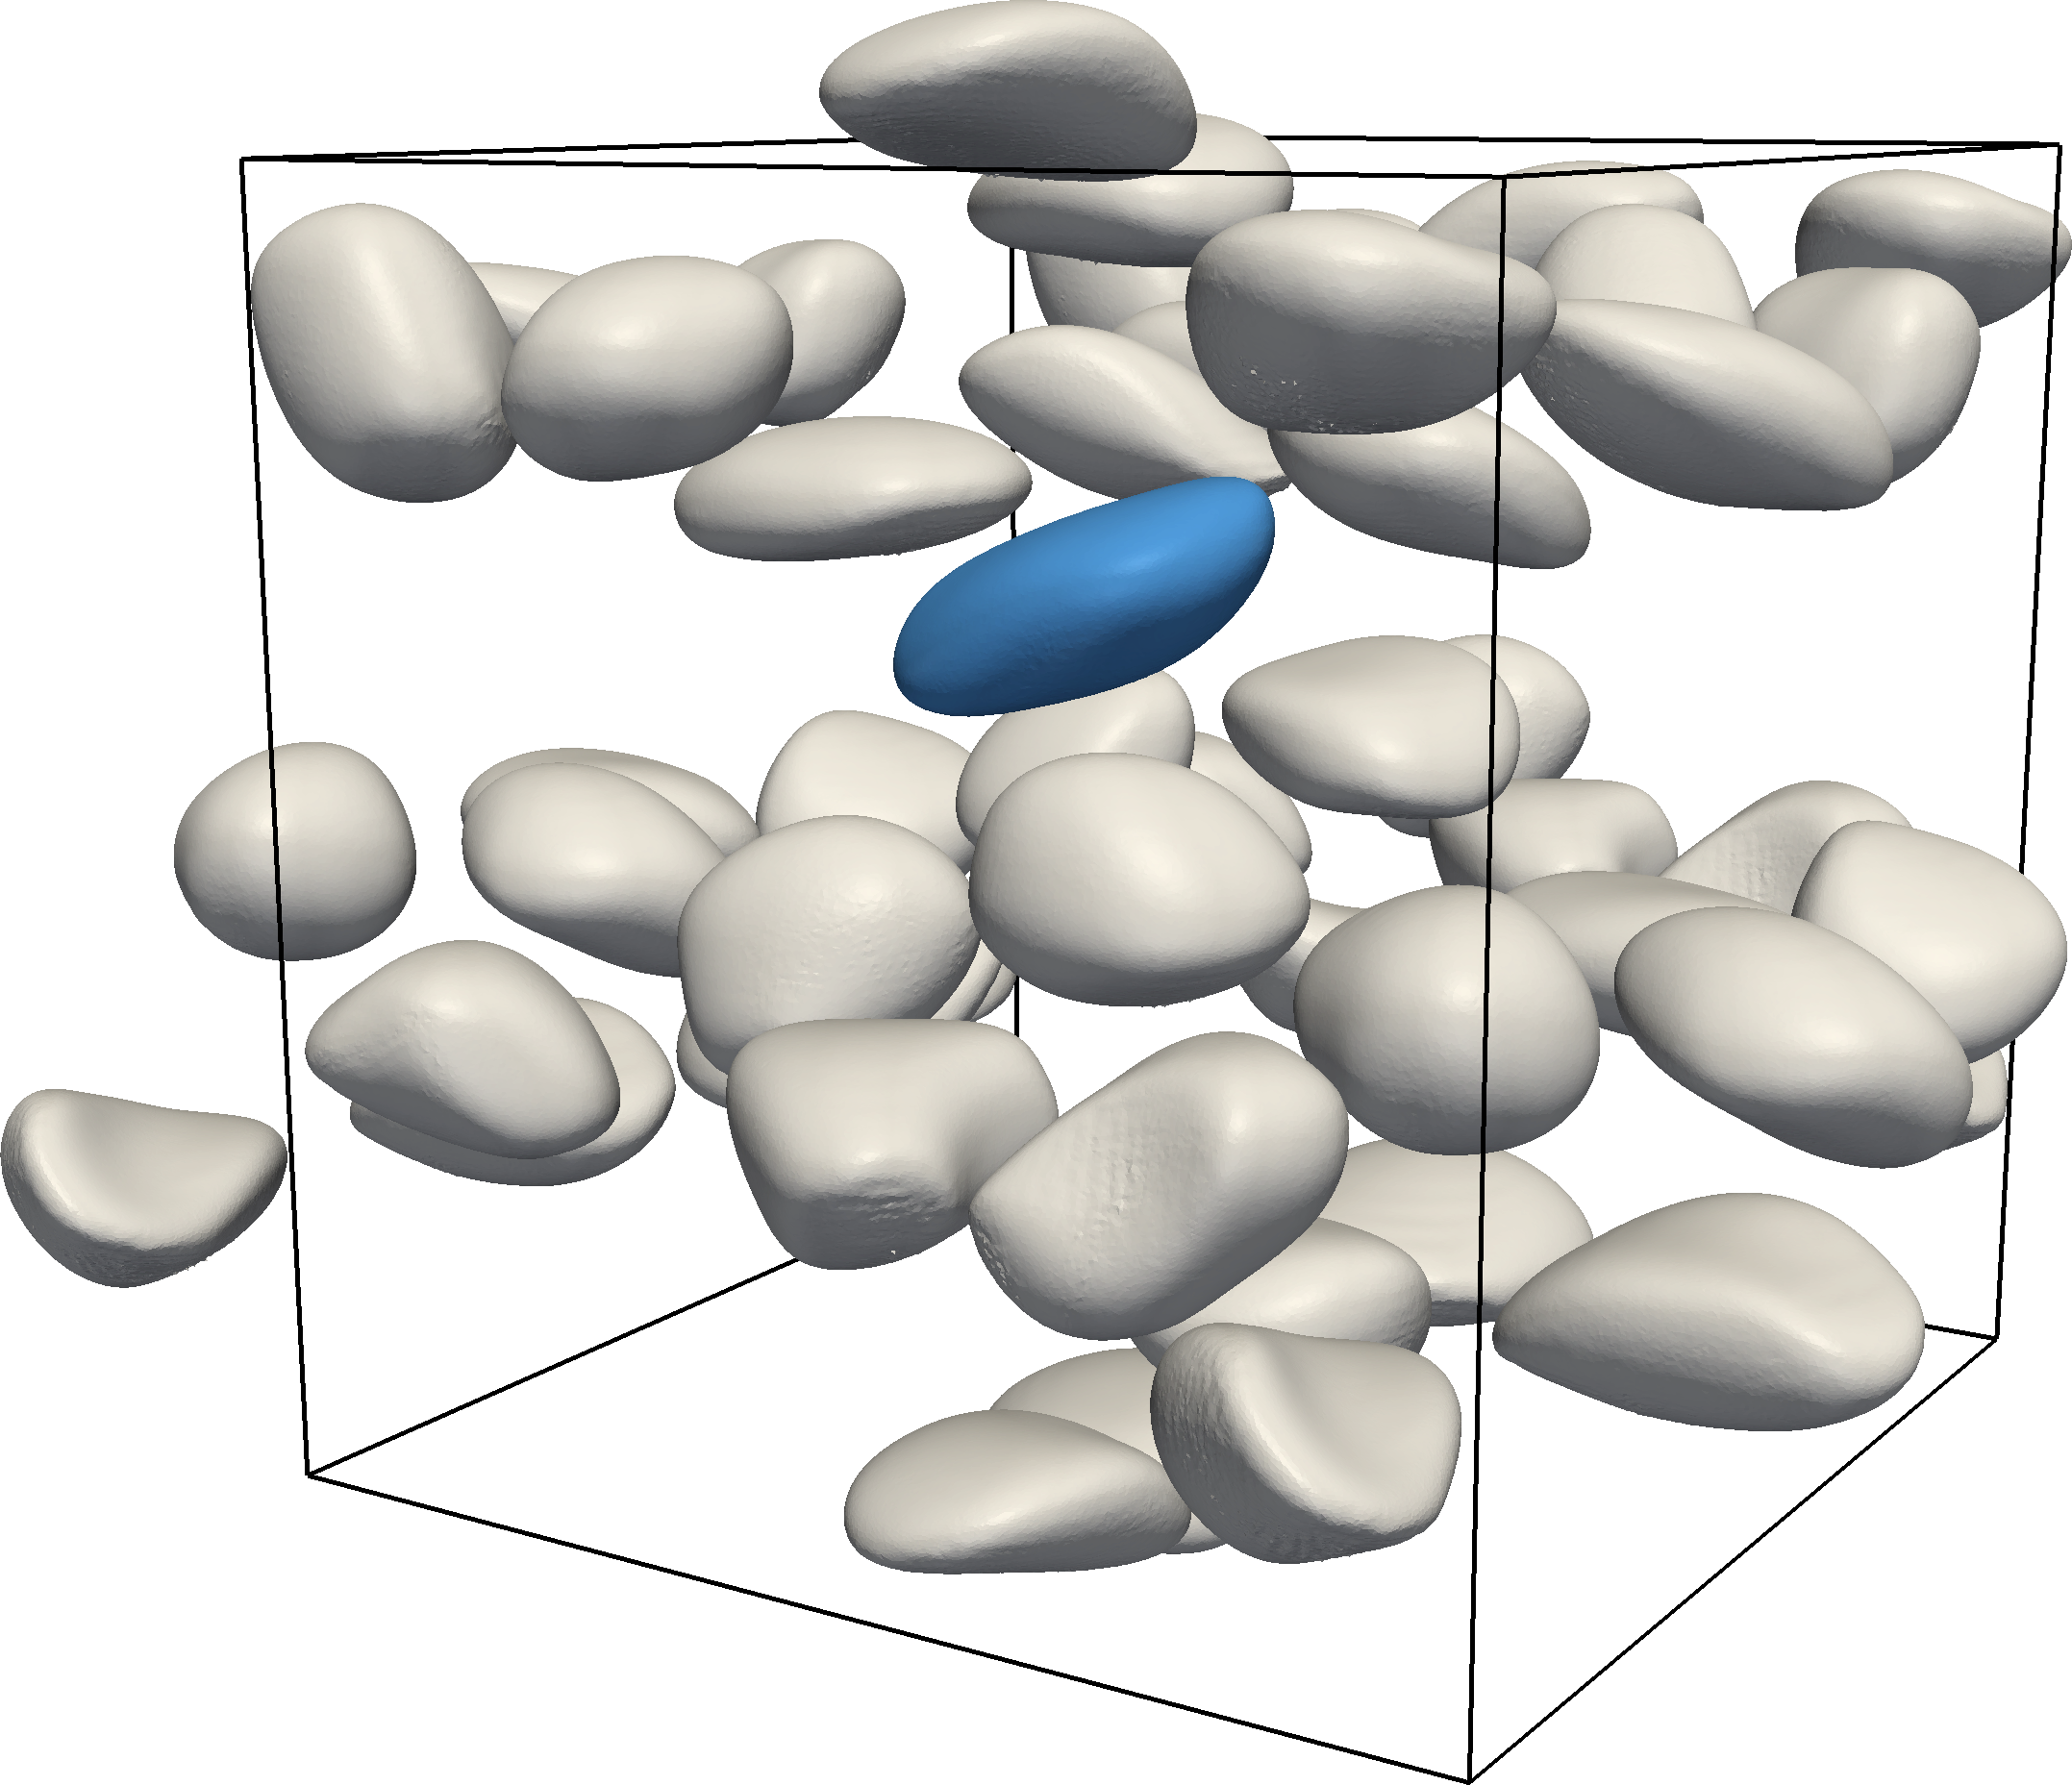
\includegraphics[width=\columnwidth]{img/sim1.png}
               };
           }]{};
  \column<2->{0.23\textwidth}
  \tikz\node[circle,draw,very thick,maincolor,
           text=white,minimum size=\columnwidth,
           path picture={
               \node at (path picture bounding box.center){
                   
\includegraphics[width=1.1\columnwidth]{img/automate.jpg}
               };
           }]{};
  \column<3->{0.23\textwidth}
  \tikz\node[circle,draw,very thick,maincolor,
           text=white,minimum size=\columnwidth,
           path picture={
               \node at (path picture bounding box.center){
                   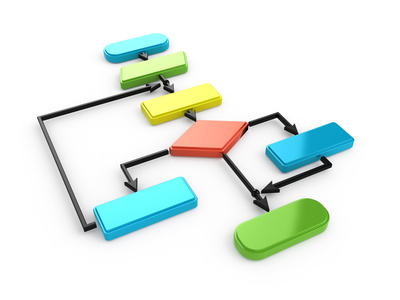
\includegraphics[width=1.2\columnwidth]{img/algorithm.jpg}
               };
           }]{};
  \column<4>{0.23\textwidth}
  \tikz\node[circle,draw,very thick,maincolor,
           text=white,minimum size=\columnwidth,
           path picture={
               \node at (path picture bounding box.center){
                   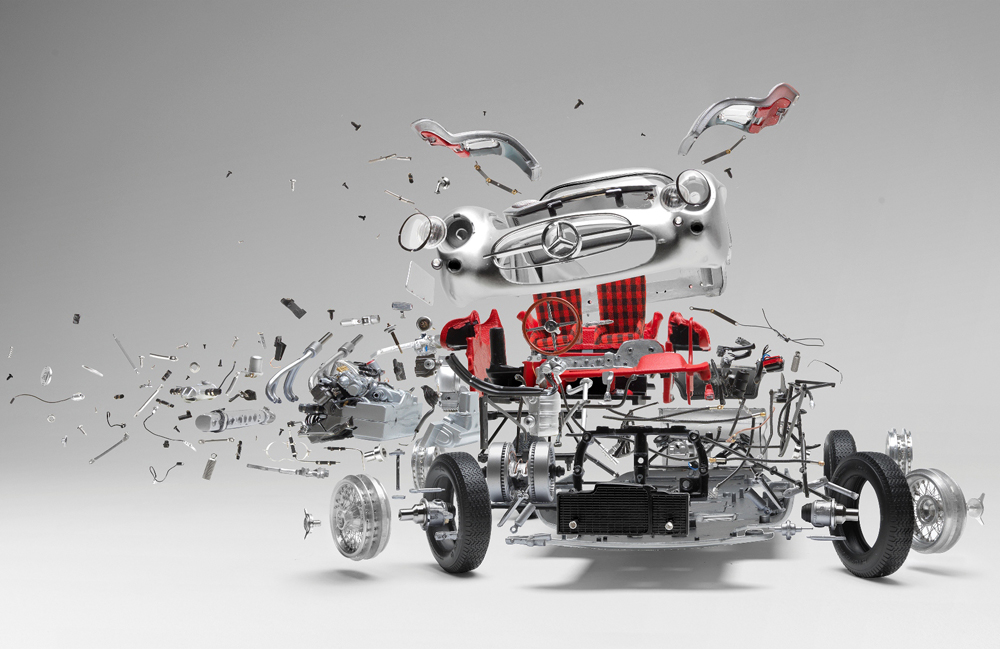
\includegraphics[width=1.5\columnwidth]{img/dissect.jpg}
               };
           }]{};
 \end{columns}

\end{frame}

\begin{frame}
 \frametitle{Introduction to programming}
 \begin{block}{What is a program?}
  \emph{A program is a sequence of instructions that is written to perform a certain task on a computer.} % SOURCE http://www.greenteapress.com/thinkpython/html/thinkpython002.html
  \end{block}
  \begin{itemize}
    \item The computation might be something mathematical, such as solving a system of equations or finding the roots of a polynomial
    \item It can also be a symbolic computation, such as searching and replacing text in a document 
    \item A program may even be used to compile another program
    \item A program consists of one or more \emph{algorithms}
  \end{itemize}
\end{frame}

\begin{frame}
 \frametitle{Getting started}
 \begin{itemize}
   \item Use an \emph{integrated development environment}
   \begin{itemize}
     \item Matlab
     \item MS Visual Studio
     \item Eclipse
     \item Dev C++
     \item IDLE, Canopy (express)
   \end{itemize}
   \item Create a simple program:
   \begin{itemize}
     \item Hello world
     \item Find the roots of a parabola
     \item Find the greatest common divisor of two numbers
   \end{itemize}
 \end{itemize}
\end{frame}

\begin{frame}
 \frametitle{Some often used programming languages}
 \fontsize{7.2pt}{7.2}\selectfont
 \begin{columns}[T]
   \column{0.45\textwidth}
   \begin{block}<1->{Python}
     \begin{itemize}
       \item Many functionalities available
       \item Smooth learning curve
       \item Slow compared to compiled languages
       \item Many freely available editors
     \end{itemize}
   \end{block}
    \begin{block}<2->{Pascal}
     \begin{itemize}
       \item Limited number of libraries available
       \item Steep learning curve
       \item Compiled language, may be fast
       \item Some free compilers (fpc)
     \end{itemize}
   \end{block}
   \column{0.45\textwidth}
   \begin{block}<3->{C / C++ / C\#}
     \begin{itemize}
       \item Many functionalities available 
       \item Steeper learning curve
       \item Needs compilation, very fast (HPC)
       \item Freely available (gcc, MSVC)
     \end{itemize}
   \end{block}

   \begin{block}<4->{Spreadsheet (Excel,LibreOffice Calc, ...)}
     \begin{itemize}
       \item High availability
       \item Low learning curve
       \item Very limited for larger problems, unbeatable for quick calculations
       \item Not always free
     \end{itemize}
   \end{block}
 \end{columns}
    \begin{block}<5>{Matlab}
     \begin{columns}[T]
     \column{0.5\textwidth}
     \begin{itemize}
       \item Many functionalities built-in (80+ toolkits!)
       \item Slow compared to compiled languages
       \end{itemize}
       \column{0.5\textwidth}
       \begin{itemize}
       \item Fairly smooth learning curve
       \item Needs a license (alternatives: SciLab, GNU Octave)
     \end{itemize}
     \end{columns}
   \end{block}
\end{frame}

\begin{frame}
\frametitle{Versatility of Matlab}
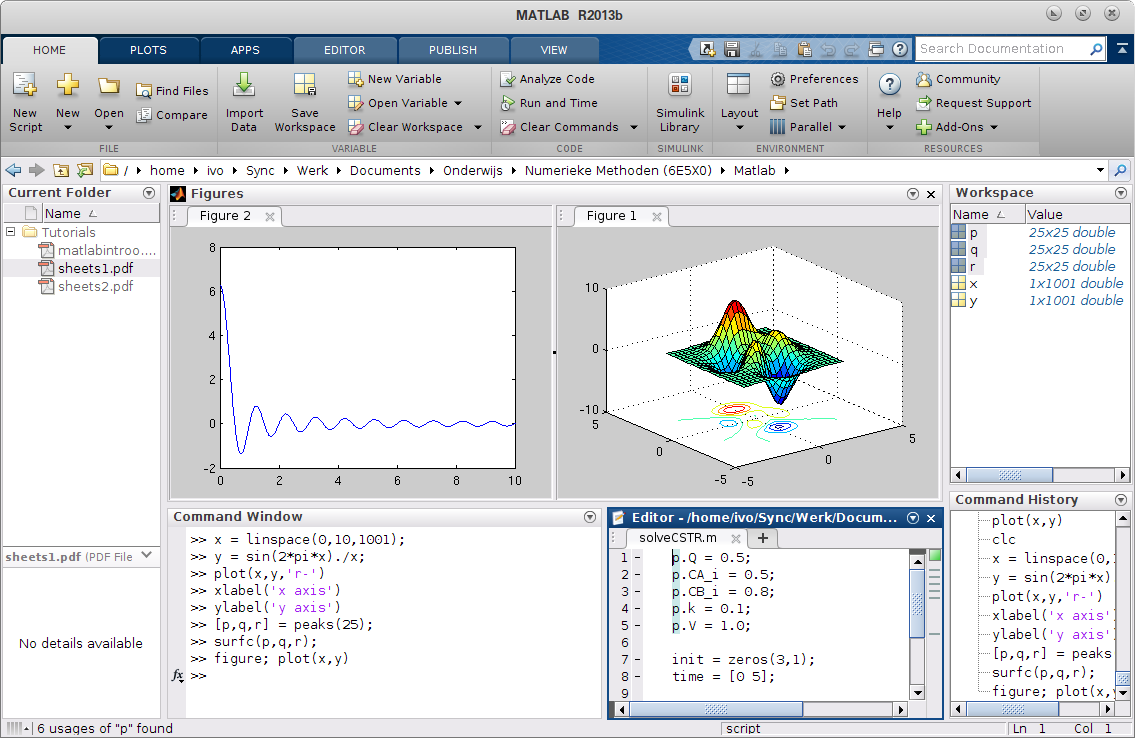
\includegraphics[width=\textwidth]{matlab.png}
\end{frame}

\begin{frame}
\frametitle{Versatility of Matlab: ODE solver}
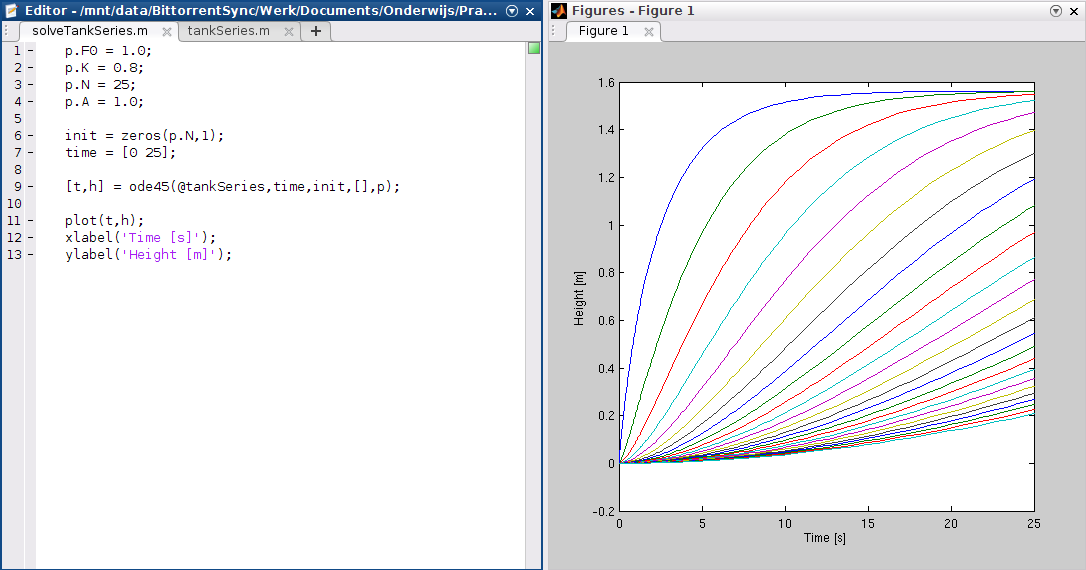
\includegraphics[width=\textwidth]{odesol.png}
\end{frame}

\begin{frame}[fragile]
\frametitle{Versatility of Matlab: Image analysis}
\begin{columns}
  \column{0.5\textwidth}
\begin{lstlisting}
I = imread('bubbles.png');
BW = rgb2gray(I);
E = edge(BW, 'canny');
F = imfill(E, 'holes');
result = regionprops(F);
\end{lstlisting}  
\column{0.5\textwidth}
  \vfill
  \includegraphics<1>[width=\columnwidth]{bub1.png}
  \includegraphics<2>[width=\columnwidth]{bub2.png}
  \includegraphics<3>[width=\columnwidth]{bub3.png}
  \includegraphics<4>[width=\columnwidth]{bub4.png}
\end{columns}
\end{frame}

\begin{frame}
\frametitle{Versatility of Matlab: Curve fitting}
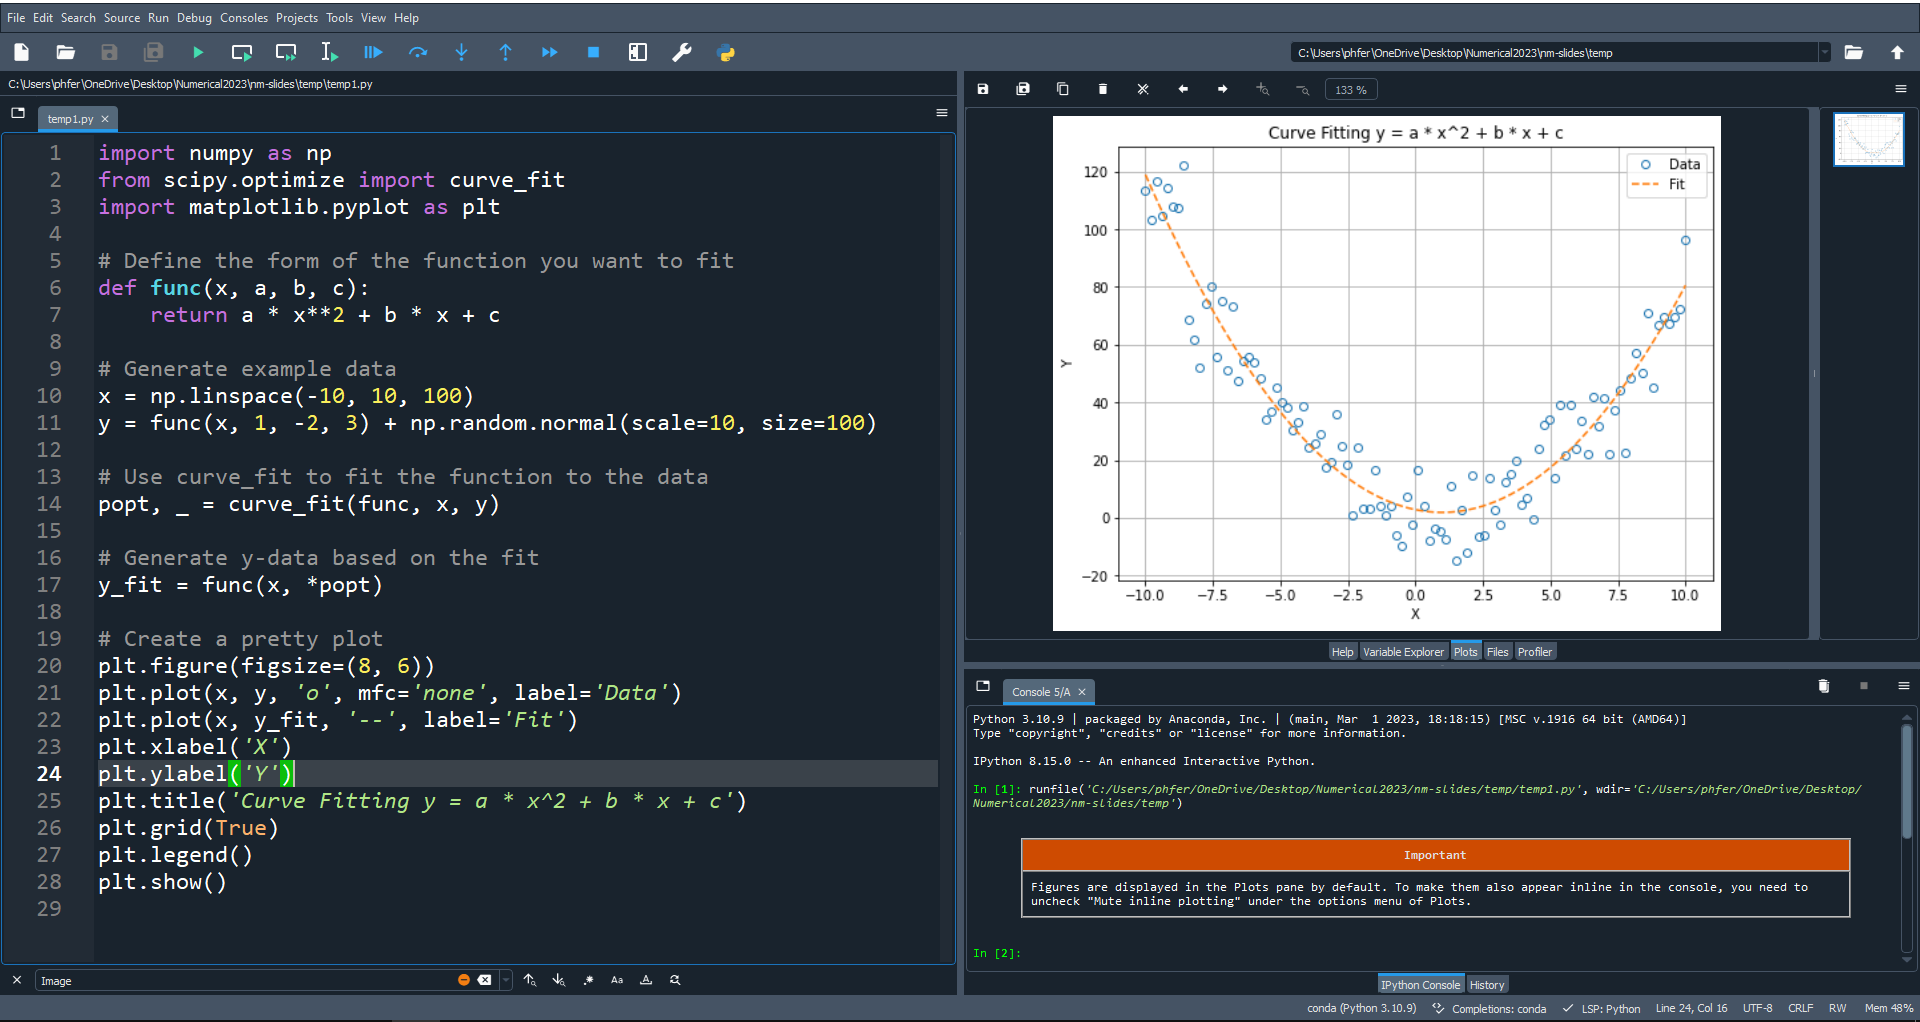
\includegraphics[width=\textwidth]{cftool.png}
\end{frame}

\begin{frame}
\frametitle{Matlab help}
\begin{itemize}[<+->]
  \item Matlab documentation: \lstinline$doc$ or \lstinline$help$ function
  \item Canvas page
  \item Introduction to Numerical Methods and Matlab Programming for Engineers. Todd Young and Martin J. Mohlenkamp (2015). GNU-licensed document, online
  \item Interactive Matlab Course. Pieter van Zutven (2010). See also \url{http://www.imc.tue.nl/}
  \item Search the web!
\end{itemize}
\vspace{-2em}
\flushright\tikz{\node[] at (4cm,-2cm) {
\includegraphics[width=0.5\textwidth]{img/help.jpg}};}
\end{frame}
%
\section{Variables}
\subsection*{Introduction}
\againframe<2>{contents}
\begin{frame}
 \frametitle{Terminology}
 \begin{description}
  \item[Variable] Piece of data stored in the computer memory, to be referenced and/or manipulated
  \item[Function] Piece of code that performs a certain operation/sequence of operations on given input
  \item[Operators] Mathematical operators (e.g. \lstinline$ + - *$ or \lstinline$/$), relational (e.g. \lstinline$< >$or \lstinline$==$, and logical operators (\lstinline$&&$, \lstinline$||$)
  \item[Script] Piece of code that performs a certain sequence of operations without specified input/output
  \item[Expression] A command that combines variables, functions, operators and/or values to produce a result.
 \end{description}
\end{frame}

\subsection*{Variables}
\begin{frame}[fragile]
 \frametitle{Variables in Matlab}
  \begin{itemize}
   \item Matlab stores variables in the \emph{workspace}\pause
   \item You should recognize the difference between the \emph{identifier} of a variable (its name, e.g. \lstinline$x$, \lstinline$setpoint_p$), and the data that it actually stores (e.g. 0.5)\pause
   \item Matlab also defines a number of variables by default, e.g. \lstinline$eps$, \lstinline$pi$ or \lstinline$i$.\pause
   \item You can assign a variable by the \lstinline$=$ sign:
   \begin{lstlisting}
>> x = 4*3
x =
    12
   \end{lstlisting}\pause
   \item If you don't assign a variable, it will be stored in \lstinline$ans$
   \item Clearing the workspace is done with \lstinline$clear$.
 \end{itemize}
\end{frame}

\begin{frame}[fragile]
  \frametitle{Vectors in Matlab (1)}
  A row vector:
  \begin{lstlisting}
>> v = [0 1 2 3]
  \end{lstlisting}\pause
  A column vector by separating elements with semi-colons:
  \begin{lstlisting}
>> u = [9; 10; 11; 12; 13]
  \end{lstlisting}\pause
  Access (i.e. read) an entry in a vector:
  \begin{lstlisting}
>> u(2)
  \end{lstlisting}\pause
  Manipulate the value of that entry:
  \begin{lstlisting}
>> u(2)=47
  \end{lstlisting}\pause
  Extract a slice out of a vector:
  \begin{lstlisting}
>> u([2 3 4]) % With colon operator: u(2:4)
  \end{lstlisting}\pause
  Transposing vectors:
  \begin{lstlisting}
>> w = v'
  \end{lstlisting}
\end{frame}

\begin{frame}[fragile]
  \frametitle{Vectors in Matlab (2)}
  Manual definition may be cumbersome. We can also use:
  \begin{lstlisting}
>> x = -1:.1:1
  \end{lstlisting}\pause
  Or, when you prefer to set the \emph{number of elements} instead of the step size:
  \begin{lstlisting}
>> y = linspace(0,10,11)
  \end{lstlisting}\pause
  Manipulating multiple components:
  \begin{lstlisting}
>> y([1 4:7]) = 1
  \end{lstlisting}\pause
  Or (by supplying a vector instead of a scalar):
  \begin{lstlisting}
>> y([1 4:7]) = 16:20 % equivalent to y[1 4 5 6 7])
  \end{lstlisting}\pause
  Removing an element:
  \begin{lstlisting}
>> size(y)
>> y(2) = []
>> size(y)
  \end{lstlisting}
\end{frame}

\begin{frame}[fragile]
  \frametitle{Printing results}
  You can prevent displaying the outcome of a command by adding a semi-colon at the end of a line:
  \begin{lstlisting}
>> c = linspace(0,10,11);
  \end{lstlisting}\pause
  Altering the display format can be done using the \lstinline$format$ command:
  \begin{lstlisting}
>> format compact % loose
>> format long    % short
  \end{lstlisting}
\end{frame}

\begin{frame}[fragile]
  \frametitle{Simple plotting}
  Make a plot of the following table
   \begin{longtable}{l!{\vrule}ccccc}
%    \rowcolors[]{1}{maincolor!20}{maincolor!10}
      T ($^\circ$C) & 5   &  20  & 30   & 50   & 55 \\
      $\mu$ (Pa$\cdot$s)  & 0.08& 0.015& 0.009& 0.006& 0.0055 \\
    \end{longtable} \pause
  \begin{lstlisting}
>> x = [ 5 20 30 50 55 ]
>> y = [ 0.08 0.015 0.009 0.006 0.0055]
\end{lstlisting}
\begin{onlyenv}<1-2>
  \begin{lstlisting}
>> plot(x,y)
  \end{lstlisting}
\end{onlyenv}
\begin{onlyenv}<3>
  \begin{lstlisting}
>> plot(x,y,'*')
  \end{lstlisting}
\end{onlyenv}
\begin{onlyenv}<4>
  \begin{lstlisting}
>> plot(x,y,'r--')
  \end{lstlisting}
\end{onlyenv}
\begin{onlyenv}<5>
  \begin{lstlisting}
>> plot(x,y,'ko-','LineWidth',2)
  \end{lstlisting}
\end{onlyenv}
\begin{lstlisting}
>> xlabel('Temperature [^\circC]')
>> ylabel('Viscosity [Pa s]')
>> title('Experiment 1')
  \end{lstlisting}
\end{frame}

\begin{frame}[fragile]
  \frametitle{Matrices in Matlab}
  Matrix A is defined as:
  \[
   \begin{bmatrix}
    8 & 1 & 6 \\
    3 & 5 & 7 \\
    4 & 9 & 2
   \end{bmatrix}\]
  In Matlab:
  \begin{lstlisting}
>> A = [ 8 1 6; 3 5 7; 4 9 2]
  \end{lstlisting}\pause
  Elements can be accessed/manipulated by the following syntax:
  \begin{lstlisting}
>> A(3,1) % Third row, first column, also A(3)
>> A(3,:) = [2 4 8] % Set entire third row
>> A(:,3) % Print third column
>> A(A>5) = 2 % Set elements by condition
  \end{lstlisting}\pause
  There are a few functions that help creating matrices:
  \begin{lstlisting}
>> A = zeros(4)  % A 4x4 matrix with zeros
>> A = ones(4,1) % A 4-element vector with ones
>> A = eye(3)    % Identity matrix of 3x3
>> A = rand(3,4) % A 3x4 matrix with random numbers
  \end{lstlisting}
\end{frame}

\begin{frame}[fragile]
 \frametitle{Datatypes and variables}
 Matlab uses different types of variables:
     \begin{longtable}{l!{\vrule}l}
      Datatype        & Example \\ \hline
      \texttt{string} & \lstinline$'Wednesday'$ \\
      \texttt{integer}& \lstinline$15$ \\
      \texttt{float}  & \lstinline$0.15$ \\
      \texttt{vector} & \lstinline$[0.0; 0.1; 0.2]$ \\
      \texttt{matrix} & \lstinline$[0.0 0.1 0.2; 0.3 0.4 0.5]$ \\
      \texttt{struct} & \lstinline$sct.name = 'MyDataName'$ \\
 \rowcolor{maincolor!20} & \lstinline$sct.number = 13$ \\
 \rowcolor{maincolor!10}\texttt{logical}& \lstinline$0$ (false)  \\
\rowcolor{maincolor!10}                      & \lstinline$1$ (true) \\
    \end{longtable}
\end{frame}

\begin{frame}[fragile]
 \frametitle{About variables}
 \begin{itemize}
   \item Matlab variables can change their type as the program proceeds (this is not common for other programming languages!):
   \begin{lstlisting}
>> s = 'This is a string'
s =
This is a string
>> s = 10
s =
    10
\end{lstlisting}
    \item Vectors and matrices are essentially \emph{arrays} of another data type. A vector of \lstinline$struct$ is therefore possible.
    \item Variables are \emph{local} to a function (more on this later).
\end{itemize}
\end{frame}

\section{Performing computations}
\subsection*{Introduction}
\begin{frame}
 \frametitle{Building blocks: Mathematics and number manipulation}
 Programming languages usually support the use of various mathematical functions (sometimes via a specialized library). Some examples of the most elementary functions in Matlab:
    \begin{longtable}{l!{\vrule}l}
      Command        & Explanation \\ \hline
      \texttt{cos(x), sin(x), tan(x)} & Cosine, sine or tangens of $x$ \\
      \texttt{mean(x), std(x)} & Mean, st. deviation of vector $x$ \\
      \texttt{exp(x)} & Value of the exponential function $e^x$ \\
      \texttt{log10(x), log(x)} & Base-10/Natural logarithm of $x$ \\
      \texttt{floor(x)} & Largest integer smaller than $x$ \\
      \texttt{ceil(x)} & Smallest integer that exceeds $x$ \\
      \texttt{abs(x)} & Absolute value of $x$ \\
      \texttt{size(x)} & Size of a vector $x$ \\
      \texttt{length(x)} & Number of elements in a vector $x$ \\
      \texttt{rem(x,y)} & Remainder of division of $x$ by $y$\\
    \end{longtable}
\end{frame}

\begin{frame}[fragile]
 \frametitle{Building blocks: conditional statements}
  \lstinline$if$-statement: Performs a block of code if a certain condition is met. \\ 
  \vskip1em \pause
  \begin{lstlisting}
num = floor (10* rand +1) ;
guess = input ('Your guess please : ') ;
if ( guess ~= num )
    disp (['Wrong, it was ', num2str(num), '. Kbye. ']) ;
else
    disp ('Correct !') ;
end
  \end{lstlisting}
  \pause
  \begin{columns}[T]
    \column{0.5\textwidth}
    Other relational operators
      \begin{longtable}{l!{\vrule}l}
      \hline
      \lstinline$==$& is equal to \\ 
      \lstinline$<=$& is less than or equal to\\
      \lstinline$>=$&is  greater than or equal to\\
      \lstinline$<$& is less than \\
      \lstinline$>$& is greater than \\
      \hline
    \end{longtable}  
    \column{0.5\textwidth}
      Combining conditional statements
      \begin{longtable}{l!{\vrule}l}
      \hline
      \lstinline$&&$& and \\ 
      \lstinline$||$& or\\
      \lstinline$xor$& exclusive or\\
      \hline
    \end{longtable}  
  \end{columns}
\end{frame}

\begin{frame}[fragile]
 \frametitle{Building blocks: loops}
  \lstinline$for$-loop: Performs a block of code a certain number of times. \\ 
  \vskip1em \pause
  \begin{lstlisting}
>> p(1) = 1;
>> p(2) = 1;
>> for i = 2:10
p(i+1) = p(i)+p(i-1);
end
>> p
p =
     1     1     2     3     5     8    13    21    34    55    89
  \end{lstlisting}
\end{frame}

\begin{frame}[fragile]
 \frametitle{Building blocks: indeterminate repetition}
  \lstinline$while$-loop: Performs and repeats a block of code until a certain condition. \\ 
  \vskip1em \pause
  \begin{lstlisting}
num = floor (10* rand +1) ;
guess = input ('Your guess please : ') ;

while ( guess ~= num )
    guess = input ('That is wrong . Try again ... ') ;
end

if (isempty(guess))
    disp('No number supplied - exit');
else
    disp ('Correct !') ;
end
  \end{lstlisting}
\end{frame}

%%%% Example
\begin{frame}[fragile]
 \frametitle{Example algorithm}
 Compute the factorial of $N$: $N! = N\cdot(N-1)\cdot(N-2)\cdots 2\cdot 1$\\ \vskip1em
 How to deal with this? \vfill
 \begin{columns}[T]
   \column{0.3\textwidth}
   \begin{block}<2->{Naive approach}
       \begin{lstlisting}
Z = 1;
Z = Z*2;
Z = Z*3;
Z = Z*4;
... etc ...      
       \end{lstlisting}
   \end{block}
   \column{0.3\textwidth}
   \begin{block}<3->{For-loop}
       \begin{lstlisting}
Z = 1;
for i = 1:N
    Z = Z*i;
end
       \end{lstlisting}
   \end{block}
   \column{0.3\textwidth}
\begin{block}<4>{While-loop}
       \begin{lstlisting}
Z = 1;
i = 1;
while (i<=N)
    Z = Z*i;
    i = i+1;
end
       \end{lstlisting}
   \end{block}
 \end{columns}
 \onslide<4>{
   Note: \lstinline$N$ must be set beforehand!\\ 
   Note: Pay attention to the relational operators!  }
\end{frame}

\begin{frame}[fragile]
 \frametitle{Building blocks: case selection}
  \lstinline$switch$-statement: Selects and runs a block of code. \\ 
  \vskip1em \pause
  \begin{lstlisting}
[dnum,dnam] = weekday(now);
switch dnum
    case {1,7}
        disp('Yay! It is weekend!');
    case 6
        disp('Hooray! It is Friday!');
    case {2,3,4,5}
        disp(['Today is ' dnam]);
    otherwise
        disp('Today is not a good day...');
end
  \end{lstlisting}
\end{frame}


\begin{frame}[fragile]
 \frametitle{Input and output}
 Many programs require some input to function correctly. A combination of the following is common:
 \begin{itemize}[<+->]
   \item Input may be given in a parameters file (``hard-coded'')
   \item Input may be entered via the keyboard
   \begin{lstlisting}
>> a = input('Please enter the number ');
   \end{lstlisting}
   \item Input may be read from a file, e.g.
    \begin{lstlisting}
>> data = getfield(importdata('myData.txt, ' ', 4), 'data');
>> numdata = xlsread('myExcelDataFile.xls');
   \end{lstlisting}
   \item There are many more advanced functions, e.g. \lstinline$fread$, \lstinline$fgets$, ...
 \end{itemize}
\end{frame}

\begin{frame}[fragile]
 \frametitle{Input and output}
 Output of results to screen, storing arrays to a file or exporting a graphic are the most common ways of getting data out of Matlab:
 \begin{itemize}[<+->]
   \item Results of each expression are automatically shown on screen as long as the line is not ended with a semi-colon;
   \item Output may be stored via the GUI:
    \begin{itemize}
      \item Use the 'Export Setup' function
      \item Save figure (use .fig, .eps or .png, \textbf{not} .jpg or .pcx)
      \item Save variables (right click, save as)
    \end{itemize}
   \item Save variables automatically (scripted):
    \begin{lstlisting}
>> savefile = 'test.mat';
>> p = rand(1,10);
>> q = ones(10);
>> save(savefile,'p','q')
   \end{lstlisting}
   \item More advanced functions can be found in e.g.  \lstinline$fwrite$, \lstinline$fprintf$, ...
 \end{itemize}
\end{frame}

\section{Functions}
\subsection*{Introduction}
\begin{frame}[fragile]
 \frametitle{Functions - general}
 A function in a programming language is a program fragment that performs a certain task. Creating functions keeps your code clean, re-usable and structured.
 \begin{itemize}
   \colorize<2-> \item You can use functions supplied by the programming language, and define functions yourself
   \colorize<3-> \item Functions take one or more input parameters (\emph{arguments}), and \emph{return} an output (result).
   \begin{itemize}
     \colorize<3-> \item If functions do not return a result, it is called a procedure
   \end{itemize}
   \colorize<4-> \item In Matlab, functions are defined as follows (2 output variables and 3 input arguments):
  \begin{overlayarea}{\textwidth}{2em}
   \begin{onlyenv}<4>
    \begin{lstlisting}
function [out1, out2] = myFunction(in1, in2, in3)
    \end{lstlisting}
    \end{onlyenv}
   \end{overlayarea}
  \end{itemize}
\end{frame}

\begin{frame}[fragile]
 \frametitle{Functions - locality and arguments}
 \begin{itemize}
   \item You are supplying arguments to a function because it does not have acces to previously defined variables. This is called \emph{locality}.
   \begin{itemize}
     \item This does not include global variables - but they're evil!
     \item Local variables created in a function are not accessible to other functions unless they are returned or supplied as an argument!
   \end{itemize}
 \end{itemize}
 \vskip1em \pause
 Exercise: write a function that takes 3 variables, and returns the average: \pause
  \begin{columns}[T]
   \column{0.5\textwidth}
   \begin{block}<2->{Approach 1}
 \begin{lstlisting}
function res = avg1(a,b,c)
    mySum = a + b + c;
    res = mySum / 3;
end \end{lstlisting}
   \end{block}
   \column{0.5\textwidth}
   \begin{block}<3->{Approach 2}
       \begin{lstlisting}
function res = avg2(a,b,c)
    data = [a; b; c];
    res = mean(data);
end \end{lstlisting}
   \end{block}
 \end{columns}
\end{frame}

\begin{frame}[fragile]
 \frametitle{Exercise: create a function}
 Compute $N! = N\cdot(N-1)\cdot(N-2)\cdots 2\cdot 1$\\ \vskip1em
 Create a function of our while-loop approach with N the argument: \\
 
 \begin{columns}[T]
   \column{0.5\textwidth}
   \begin{block}{Original script}
	   \begin{lstlisting}
Z = 1;
i = 1;
while (i<=N)
    Z = Z*i;
    i = i+1;
end \end{lstlisting}
   \end{block}
   \column{0.5\textwidth}
   \begin{block}<2>{Function}
	   \begin{lstlisting}
function Z = fact_while(N)

Z = 1;
i = 1;
while (i<=N)
    Z = Z*i;
    i = i+1;
end

end
	   \end{lstlisting}
   \end{block}
 \end{columns}
\end{frame}

\begin{frame}[fragile]
 \frametitle{Functions - checking input}
  The function we created computes the factorial correctly! \pause
  \begin{itemize}
     \item When the supplied argument is positive\pause\ and \pause
     \item When the supplied argument is a natural number...
  \end{itemize}\pause
  \begin{columns}[T]
   \column{0.4\textwidth}
     
\includegraphics[width=\columnwidth]{deadmau5.png}
   \column{0.6\textwidth}
    \pause
    \begin{itemize}[<+->]
     \item In this case, we should check the user input to prevent an infinite loop: \pause
     \begin{lstlisting}
if (fix(N)~=N) | (N<0)
    disp 'Provide a positive integer number!'
    return;
end \end{lstlisting}
      \item If no check can be done before a while-loop, you may want to stop after $x$ loops
    \end{itemize}
  \end{columns}
\end{frame}

\begin{frame}[fragile]
 \frametitle{Functions - checking input}
  The whole factorial function, including comments:
     \begin{lstlisting}
function Z = fact_while(N)
%% This function computes a factorial of input value N
% Usage  : fact_while(N)
% N      : value of which the factorial is computed
% returns: factorial of N

% Catch non-integer case
if (fix(N)~=N) | (N<0)
    disp 'Provide a positive integer number!'
    return;
end

Z = 1;
i = 1;
while (i<=N)
    Z = Z*i;
    i = i+1;
end

end \end{lstlisting}
\end{frame}

\begin{frame}[label=recursion,fragile]
 \frametitle{Recursion}
 \begin{columns}
   \column{0.5\textwidth}
   \begin{itemize}
    \item<1-> In order to understand recursion, one must first understand recursion
    \item<2-> A recursive function is called by itself (a function within a function)
    \begin{itemize}
      \item<3-> This could lead to infinite calls;
      \item<3-> A base case is required so that recursion is stopped;
      \item<3-> Base case does not call itself, simply returns.
    \end{itemize}
 \end{itemize}
   \column{0.5\textwidth}
   \includegraphics<3>[width=0.8\columnwidth]{inception.jpg}
 \end{columns}
\end{frame}

\againframe{recursion}

\begin{frame}[fragile]
 \frametitle{Recursion: example}
 \begin{lstlisting}
function out = mystery(a,b)
if (b == 1)
    % Base case
    out = a;
else 
    % Recursive function call
    out = a + mystery(a,b-1);
end
 \end{lstlisting}
\vskip1em \pause
\begin{itemize}
  \item What does this function do? \pause
  \item Can you spot the error? \pause
  \item How deep can you go? Which values of b don't work anymore?
\end{itemize}
\end{frame}

\begin{frame}[fragile]
 \frametitle{Recursion: exercise}
 Create a function computing the factorial of $N$, based on recursion. \pause
 \begin{lstlisting}
function res = fact_recursive(x)

% Catch non-integer case
if (fix(x)~=x) | (x<0)
    disp 'You should provide a positive integer number only'
    return;
end

if (x > 1)
    res = x*fact_recursive(x-1);
else
    res = 1;
end

end 
 \end{lstlisting}
\end{frame}

\part{Advanced Programming techniques}
\frame{\partpage}

\section{Code style}
\subsection*{Introduction}
\begin{frame}[fragile]
 \frametitle{Interpret the following code}
 \begin{lstlisting}
s=checksc();
if(s==true)
a=cb();
b=cfrsp();
if(a<5)
if(b>5)
a=gtbs();
end
if(a>b)
ubx();
end
end
else
brn();
gtbs();
end
 \end{lstlisting}
\end{frame}


\section{Eliminating errors}
\againframe<2>{contents}
\subsection*{Errors in programming}
\againframe<2>{contents}
\begin{frame}
 \frametitle{Errors in computer programs}
 \begin{center}
    Computer programs often contain errors (bugs): buildings collapse, governments fall, kittens will die.\\
      \vskip1em
    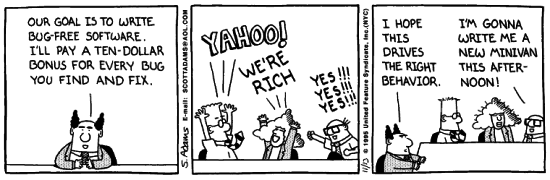
\includegraphics[width=0.8\textwidth]{bugFree.png}
 \end{center}
\end{frame}

\begin{frame}
 \frametitle{Errors in computer programs}
 \footnotesize\selectfont
 The following symptoms can be distinguished:
 \begin{itemize}
   \item Unable to execute the program
   \item Program crashes, warnings or error messages
   \item Never-ending loops
   \item Wrong (unexpected) result
 \end{itemize}
 \vskip1em
 \uncover<2->{
  Three error categories:
  \begin{description}
   \colorize<2->  \item[Syntax errors] You did not obey the language rules. These errors prevent running or compilation of the program.
   \colorize<3->  \item[Runtime errors] Something goes wrong during the execution of the program resulting in an error message (problem with input, division by zero, loading of non-existent files, memory problems, etc.)
   \colorize<4->  \item[Semantic errors] The program does not do what you expect, but does what have told it to do.
  \end{description}
 }
\end{frame}

\begin{frame}[fragile]
 \frametitle{Verification and validation}
  \scriptsize\selectfont
  \begin{columns}
    \column{0.6\textwidth}
    \uncover<3->{\begin{block}{Verification}
    Verification is the process of mathematically and computationally assuring that the model computes what you have entered.    
    \end{block}
    }
    \uncover<7->{
    \begin{block}{Validation}
      Validation is the process of determining the degree to which a model is an accurate representation of the real world from the perspective of the intended uses of the model
    \end{block}
    }

  \column{0.4\textwidth}
    \begin{tikzpicture}[block/.style={rectangle,minimum size=3mm,text badly centered,drop shadow,
					thick,rounded corners,draw=maincolor,top color=maincolor!35,bottom color=maincolor!20,
					font=\sffamily\scriptsize},>=stealth,node distance=0.75cm]
	\node[block] (p) at (0,0) {Problem};
	\uncover<2->{\node[below of=p] (p1) {};
	\node[block, below of=p1] (mm) {Mathematical Model};
	\node[below of=mm] (mm1) {};}
	\uncover<4->{\node[block, below of=mm1] (cm) {Computational Model};
	\node[below of=cm] (cm1) {};}
	\uncover<6->{\node[block, below of=cm1] (r) {Results};}
	
	\uncover<3->{\node[block, left of=p1,node distance=2cm] (v1) {Verification};}
	\uncover<5->{\node[block, left of=mm1,node distance=2cm] (v2) {Verification};}
	\uncover<7->{\node[block, left of=cm1,node distance=2cm] (v3) {Validation};}
	
	\uncover<2->{\draw[->] (p) -> (mm);}
	\uncover<4->{\draw[->] (mm) -> (cm);}
	\uncover<6->{\draw[->] (cm) -> (r);}
	
	\uncover<3->{\draw[->] (v1) -> (p1);}
	\uncover<5->{\draw[->] (v2) -> (mm1);}
	\uncover<7->{\draw[->] (v3) -> (cm1);}
    \end{tikzpicture}
  \end{columns}

\end{frame}
% 

\begin{frame}
  \frametitle{Be aware of your uncertainties}
  \scriptsize\selectfont
  \begin{columns}
    \column{0.5\textwidth}
    \begin{center}
      \mode<beamer>{
	\includegraphics<1>[width=0.8\columnwidth]{ptolemy1-1}
	\includegraphics<2>[width=0.8\columnwidth]{ptolemy1-2}
	\includegraphics<3>[width=0.8\columnwidth]{ptolemy1-3}
	\includegraphics<4>[width=0.8\columnwidth]{ptolemy1-4}
	\includegraphics<5>[width=0.8\columnwidth]{ptolemy1-5}
	\includegraphics<6>[width=0.8\columnwidth]{ptolemy1-6}
      }
      \includegraphics<7->[width=0.8\columnwidth]{ptolemy1-7}
    \end{center}
    \column{0.5\textwidth}
    \begin{center}
      \mode<beamer>{
	\includegraphics<7>[width=0.8\columnwidth]{ptolemy2-0}
	\includegraphics<8>[width=0.8\columnwidth]{ptolemy2-1}
	\includegraphics<9>[width=0.8\columnwidth]{ptolemy2-2}
	\includegraphics<10>[width=0.8\columnwidth]{ptolemy2-3}
	\includegraphics<11>[width=0.8\columnwidth]{ptolemy2-4}
	\includegraphics<12>[width=0.8\columnwidth]{ptolemy2-5}
	\includegraphics<13>[width=0.8\columnwidth]{ptolemy2-6}
      }
      \includegraphics<14>[width=0.8\columnwidth]{ptolemy2-7}
    \end{center}
  \end{columns}
  \begin{itemize}
    \item<7-> The perceived orbit of Mars from Earth shows a zig-zag (in contrast to the Sun, Mercury, Venus)
    \item<14> Even though they were not 'right', Earth-centered models (Ptolemy) were still valid
  \end{itemize}
\end{frame}

\begin{frame}
  \frametitle{Be aware of your uncertainties}
  \vfill
  \begin{block}{Aleatory uncertainty}
    Uncertainty that arises due to inherent randomness of the system, features that are too complex to measure and take into account
  \end{block}
  \vskip1em
  \begin{block}{Epistemic uncertainty}
      Uncertainty that arises due to lack of knowledge of the system, but could in principle be known
  \end{block}
  \vfill
\end{frame}

%  
\subsection*{Debugging}
\begin{frame}
\frametitle{A convenient tool: the debugger}
\begin{itemize}
  \colorize<1-> \item No-one can write a 1000-line code without making errors
  \begin{itemize}
    \colorize<1-> \item If you can, please come work for us
  \end{itemize}
  \colorize<2-> \item One of the most important skills you will acquire is debugging.
  \colorize<3-> \item Although it can be frustrating, debugging is one of the most intellectually rich, challenging, and interesting parts of programming.
  \colorize<4-> \item In some ways, debugging is like detective work. You are confronted with clues, and you have to infer the processes and events that led to the results you see.
\end{itemize}
\onslide<4>{
\vskip1em
\begin{raggedleft}
\emph{``When you have eliminated the impossible, whatever remains, however improbable, must be the truth.''}
\\
--- A. Conan Doyle, The Sign of Four\\ % http://www.greenteapress.com/thinkpython/html/thinkpython002.html
\end{raggedleft}
}
\end{frame}

\begin{frame}
\frametitle{A convenient tool: the debugger}
The debugger can help you to:
\begin{itemize}
  \item Pause a program at a certain line: set a \emph{breakpoint}
  \item Check the values of variables during the program
  \item Controlled execution of the program:
  \begin{itemize}
    \item One line at a time
    \item Run until a certain line
    \item Run until a certain condition is met (conditional breakpoint)
    \item Run until the current function exits
  \end{itemize}
  \item Note: You may end up in the source code of Matlab functions!
\end{itemize}
\end{frame}
% 
\begin{frame}
  \frametitle{About testcases (validation)}
  \begin{itemize}
    \item Testcases: run the program with parameters such that a known result is (should be) produced.
    \item Testcases: what happens when unforeseen input is encountered?
    \begin{itemize}
      \item More or fewer arguments than anticipated? (Matlab uses \lstinline$varargin$ and \lstinline$nargin$ to create a varying number of input arguments, and to check the number of given input arguments
      \item Other data types than anticipated? How does the program handle this? Warnings, error messages (crash), NaN or worse (a continuing program)?
    \end{itemize}
    \item For physical modeling, we typically look for analytical solutions
    \begin{itemize}
      \item Sometimes somewhat stylized cases
      \item Possible solutions include Fourier-series
      \item Experimental data
    \end{itemize}

  \end{itemize}
\end{frame}
% 
\begin{frame}
 \frametitle{Advanced concepts}
 \begin{itemize}
   \item Object oriented programming: classes and objects
   \item Memory management: some programming languages require you to allocate computer memory yourself (e.g. for arrays)
   \item External libraries: in many cases, someone already built the general functionality you are looking for
   \item Compiling and scripting (``interpreted''); compiling means converting a program to computer-language before execution. Interpreted languages do this on the fly.
   \item Profiling, optimization, parallellization: Checking where your program spends the most of its time, optimizing (or parallellizing) that part.
 \end{itemize}
\end{frame}
% 
\begin{frame}
  \frametitle{If anything sticks today, let it be this}
  \begin{center}
    {\LARGE Your code will not be understood by anyone\\}
  \pause
  \vskip1em
  That includes future-you
  \vskip2em
  \end{center}
  \pause
  This can be prevented somewhat by the following
  \begin{itemize}
    \item Use comments! In Matlab, everything following \lstinline$ \% is a comment$
    \item Prevent ``smart constructions''. You will spend a day tinkering why it does what it does...
    \item If you write unmaintainable code, you'll have a job for life.
    \item Use comments! Documentation is also useful (though hard to maintain)
  \end{itemize}
\end{frame}
% 
\section{Visualisation}
\againframe<2>{contents}
\subsection*{Plotting}
\againframe<2>{contents}
\begin{frame}
 \frametitle{Data visualisation}
 Modeling can lead to very large data sets, that require appropriate visualisation to convey your results.
 \begin{columns}
   \column{0.6\textwidth}
    \begin{itemize}
      \item 1D, 2D, 3D visualisation
      \item Multiple variables at the same time (temperature, concentration, direction of flow)
      \item Use of colors, contour lines
      \item Use of stream lines or vector plots
      \item Animations
    \end{itemize}
   \column{0.4\textwidth}
   \centering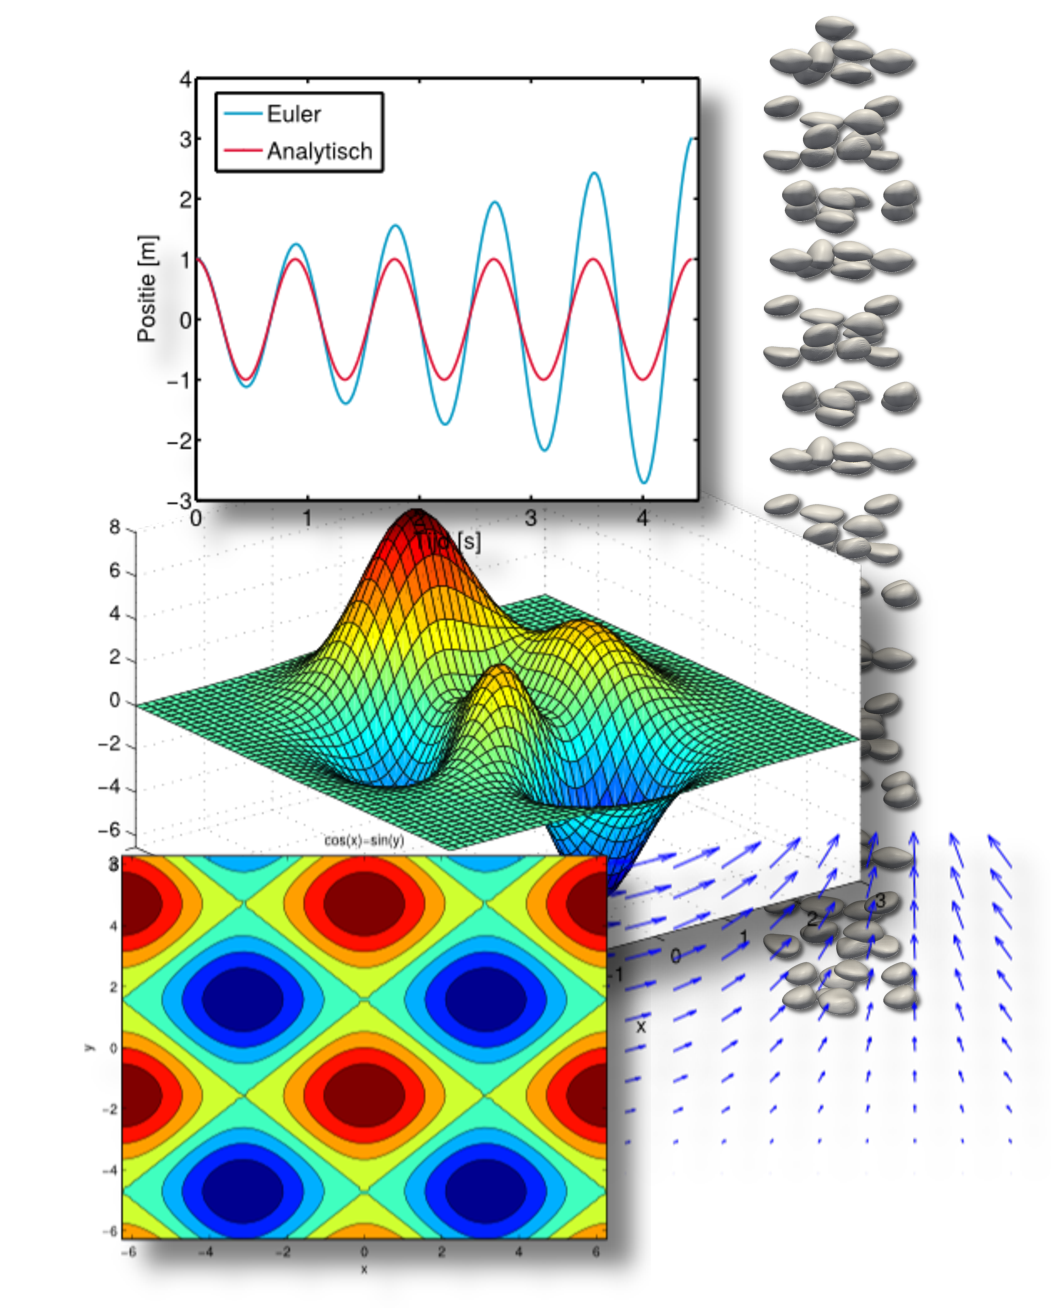
\includegraphics[width=\columnwidth]{visualisation}
 \end{columns}
\end{frame}

\begin{frame}[fragile]
  \frametitle{Plotting}
  \begin{lstlisting}
x = -5:0.1:5;
y = x.^2-4*x+3;
y2 = y + (2-4*rand(size(y)));
subplot(2,1,1); plot(x,y,'-',x,y2,'r.');
xlabel('X'); ylabel('Y'); title('Graph and scatter data');
subplot(2,1,2); plot(x,abs(y-y2),'r-');
xlabel('X'); ylabel('Y'); title('Absolute error');
  \end{lstlisting}
  \centering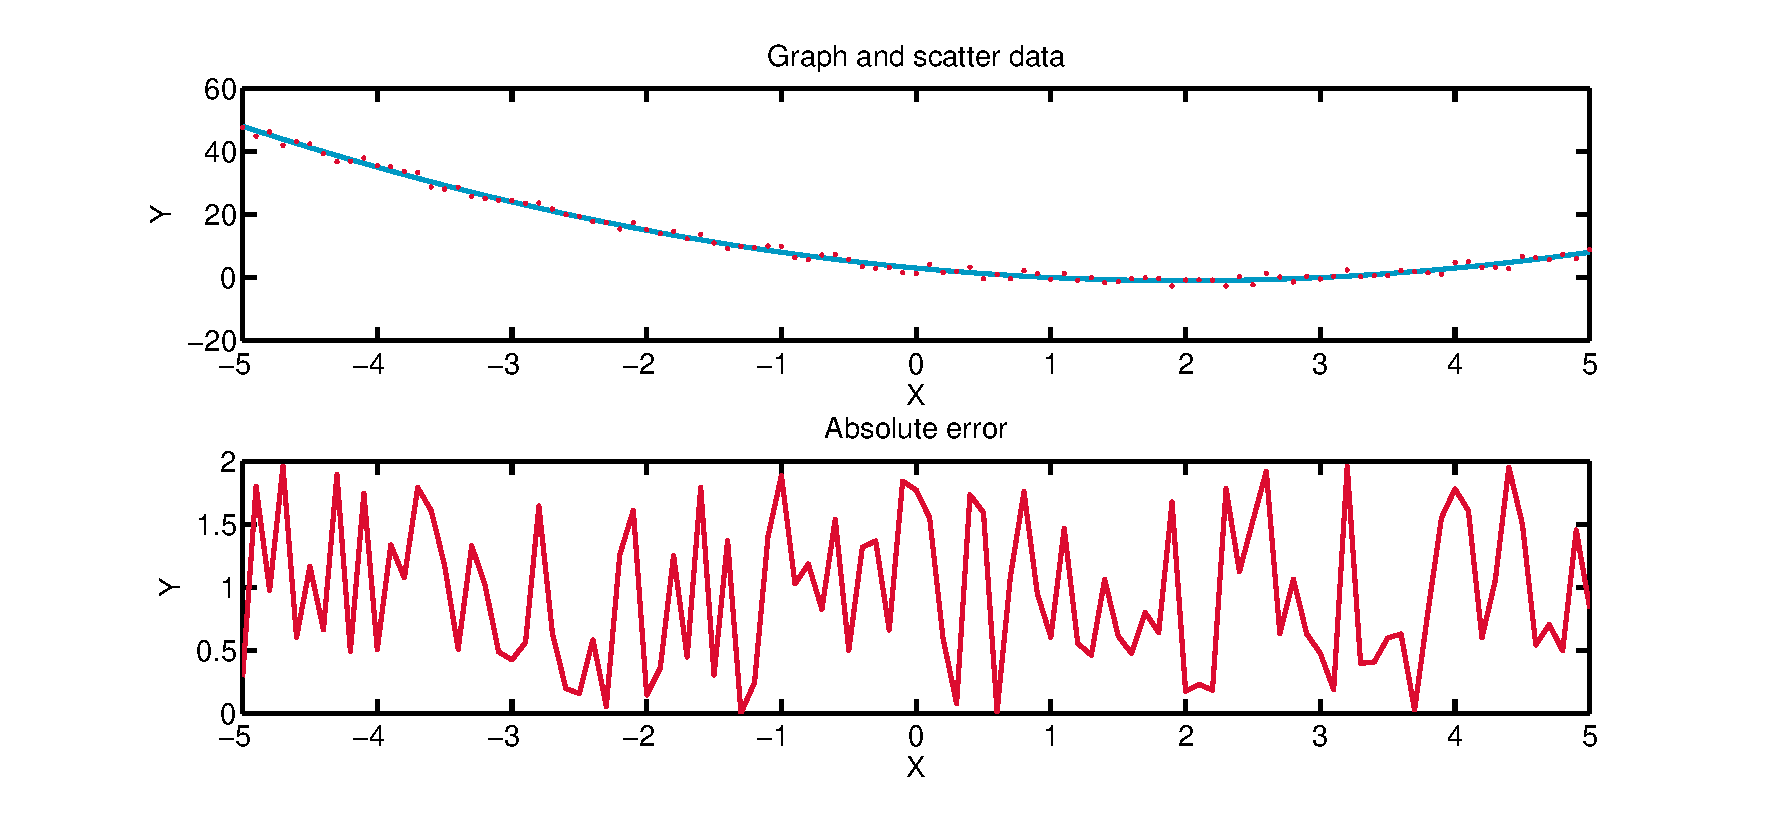
\includegraphics[width=0.8\textwidth]{showplot-utc}
\end{frame}

\begin{frame}[fragile]
  \frametitle{Plotting (2)}
  Easy plotting of functions can be done using the ezplot function: \lstinline$ezplot('x-sin(x)', [0 2*pi])$:
  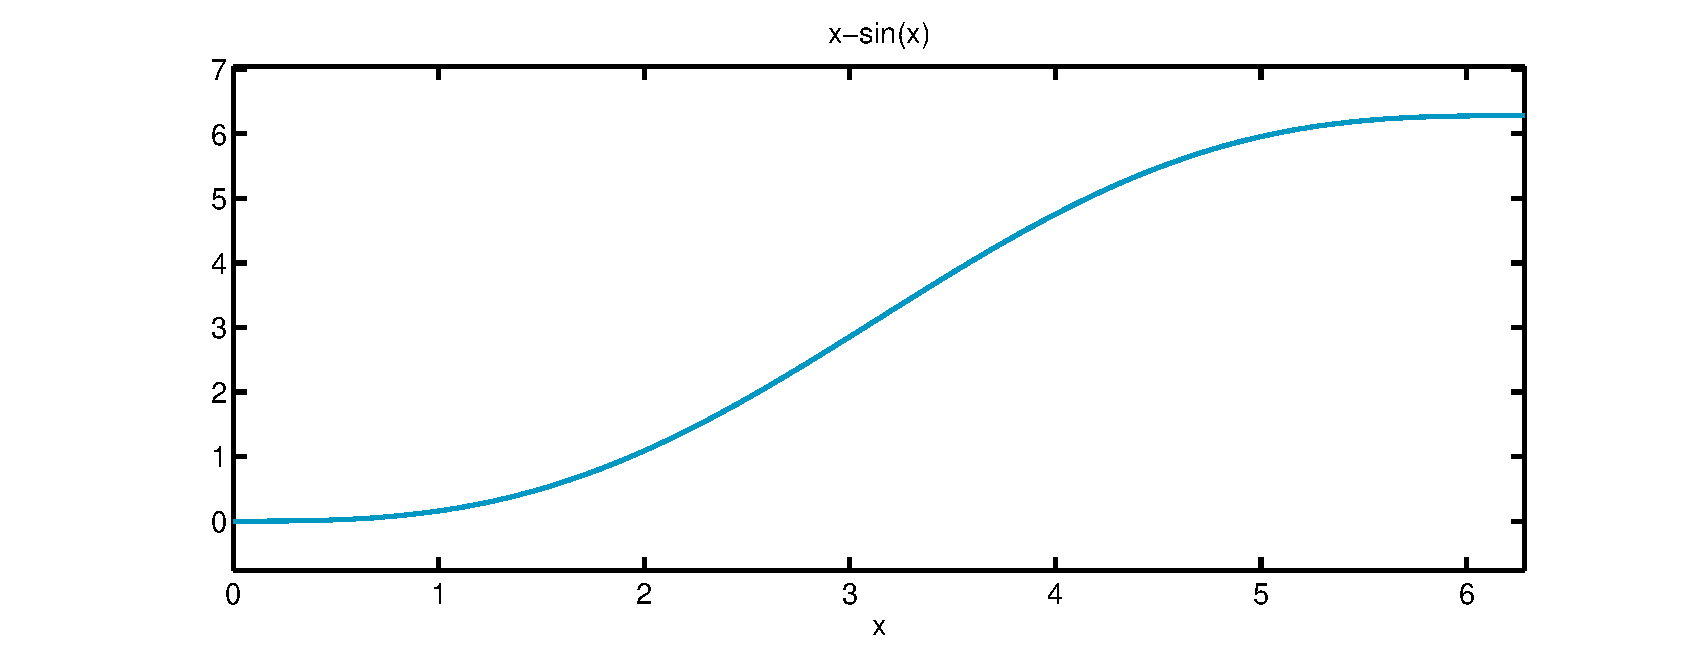
\includegraphics[width=0.7\textwidth]{show_ezplot-utc}\\
  Be careful with steep gradients: \lstinline$ezplot('x-sin(1/x)', [0 1])$% (use \lstinline$fplot$ instead)
  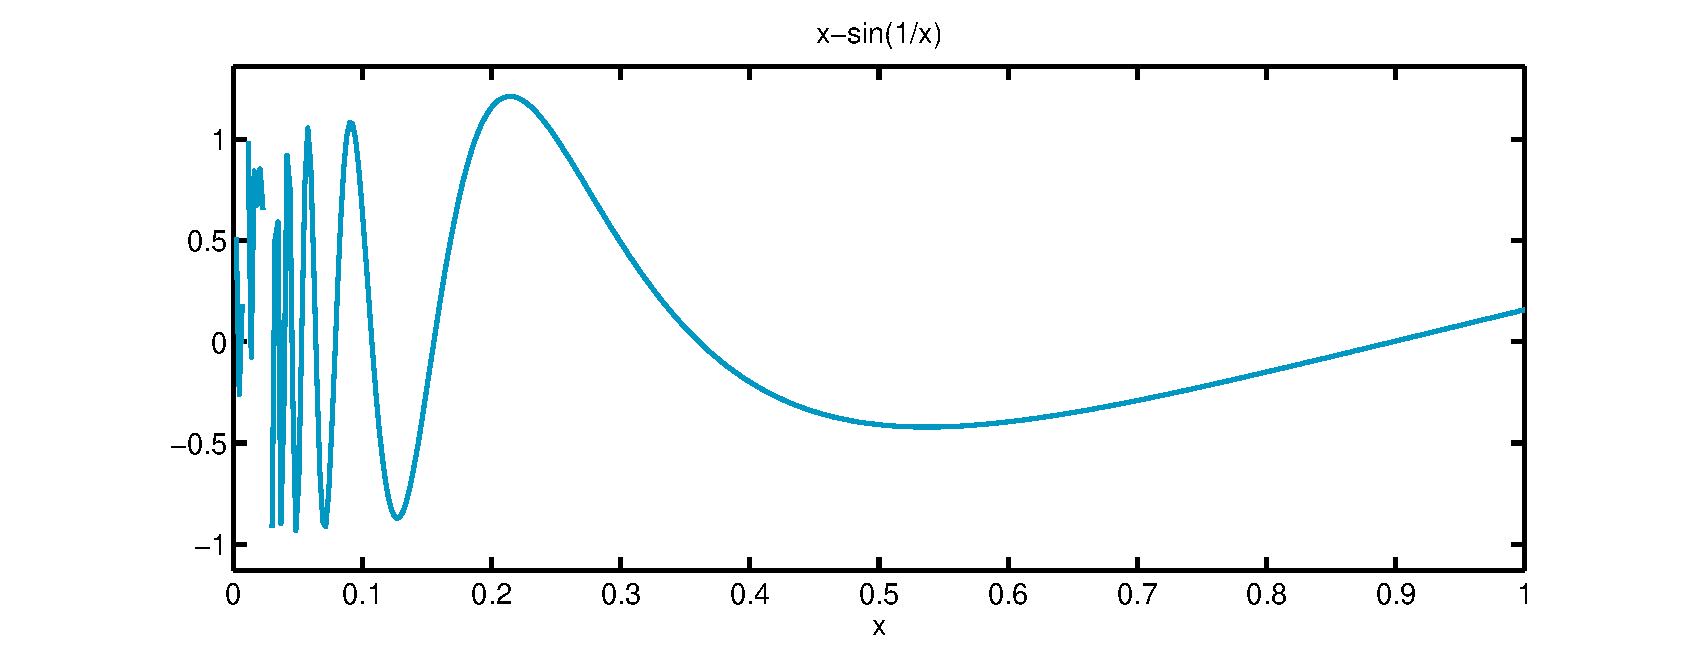
\includegraphics[width=0.7\textwidth]{show_ezplot2-utc}
\end{frame}

\begin{frame}[fragile]
  \frametitle{Other plotting tools}
  \begin{columns}
   \column{0.6\textwidth}
    \begin{itemize}[<+->]
      \item Errorbars: \lstinline$errorbar(x,y,err)$
      \item 3D-plots: \lstinline$plot3(x,y,z)$
      \item Histograms: \lstinline$histogram(x,20)$
%       \item Vectorplots: \lstinline$quiver(x,y,vx,vy)$
    \end{itemize}
   \column{0.4\textwidth}
    \includegraphics<1>[width=\columnwidth]{show_errorbar-utc}
    \includegraphics<2>[width=\columnwidth]{show_ezplot3-utc}
    \includegraphics<3>[width=\columnwidth]{show_hist-utc}
%     \includegraphics<3>[width=\columnwidth]{show_quiver-utc}
    
 \end{columns}
\end{frame}

\subsection*{Multi-dimensional data}
\begin{frame}[fragile]
  \frametitle{Multi-dimensional data}
  Matlab typically requires the definition of rectangular grid coordinates using \lstinline$meshgrid$:\\
  \begin{overlayarea}{\textwidth}{6cm}
  \begin{columns}[T]
   \column{0.6\textwidth}
    \begin{lstlisting}
[x y] = meshgrid(-2:0.1:2, -2:0.1:2);
z = x .* y .* exp(-x.^2 - y.^2);
    \end{lstlisting}
    \vskip1em
    \begin{itemize}
      \item<2-> Surface plot
      \item<3-> Contour plot
      \item<4-> Waterfall 
      \item<5> Ribbons
    \end{itemize}
   \column{0.4\textwidth}
   \begin{center}
      \includegraphics<2>[width=\columnwidth]{show_surf}
      \includegraphics<3>[width=\columnwidth]{show_contour}
      \includegraphics<4>[width=\columnwidth]{show_waterfall}
      \includegraphics<5>[width=\columnwidth]{show_ribbon}
   \end{center}
    \only<2>{
      \lstinline$surf(x,y,z);$
    }
    \only<3>{
      \lstinline$v=-0.5:0.05:0.5;$ \\
      \lstinline$contour(x,y,z,v,'ShowText', 'on');$
    }
    \only<4>{
    \lstinline$waterfall(x,y,z);$\\
    \lstinline$colormap(winter);$
    }
    \only<5>{
    \lstinline$ribbon(z);$
    }
 \end{columns}
 \end{overlayarea}
\end{frame}

\begin{frame}[fragile]
  \frametitle{Vector data}
  The gradient operator, as expected, is used to obtain the gradient of a scalar field. Colors can be used in the background to simultaneously plot field data:
  \begin{columns}[T]
   \column{0.6\textwidth}
    \begin{lstlisting}
[x y] = meshgrid(-2:0.2:2, -2:0.2:2);
z = x .* y .* exp(-x.^2 - y.^2)
[dx dy] = gradient(z,8,8)

% Background
contourf(x,y,z,30,'LineColor','none');
colormap(hot); colorbar;

axis tight; hold on;

% Vectors
quiver(x,y,dx,dy,'k');
    \end{lstlisting}
   \column{0.4\textwidth}
   \begin{center}
      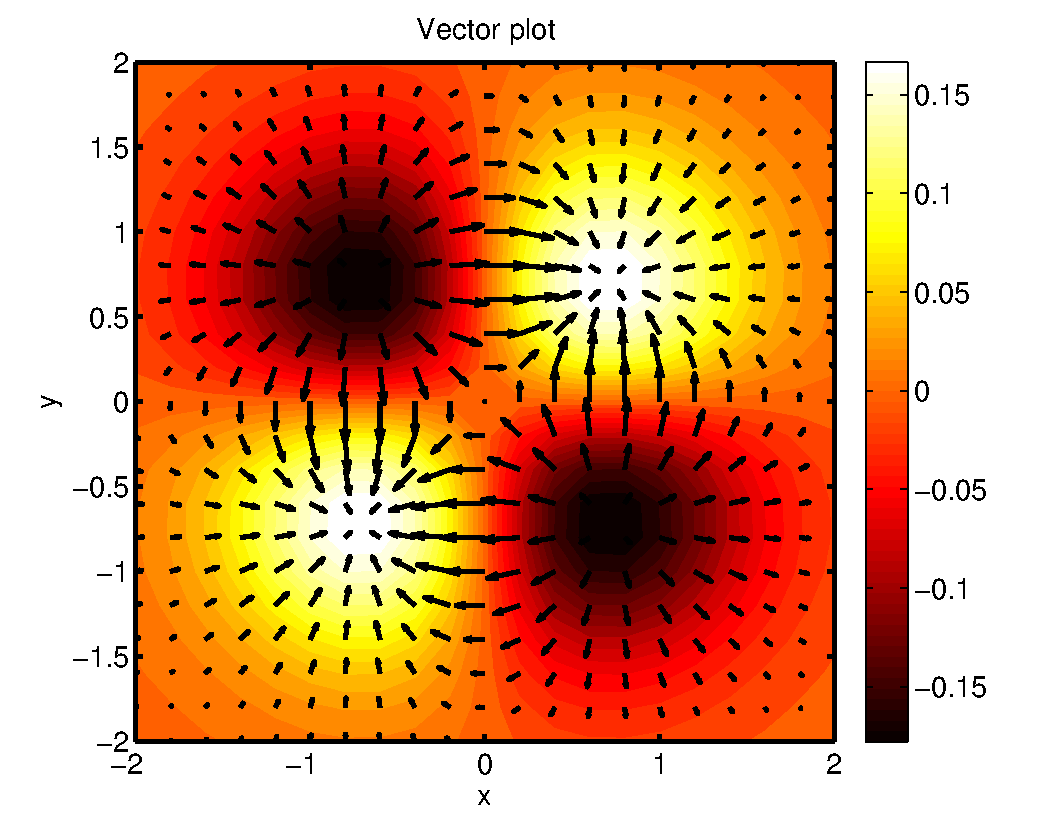
\includegraphics[width=\columnwidth]{show_vector}
    \end{center}
  \end{columns}
\end{frame}

\section{Excel}
\againframe<2>{contents}
\subsection*{Solver and goal-seek}
\begin{frame}
  \frametitle{Solver and goal-seek}
  Excel comes with a goal-seek and solver function. For Excel 2010:
  \begin{itemize}
    \item Install via Excel $\Rightarrow$ File $\Rightarrow$ Options $\Rightarrow$ Add-Ins $\Rightarrow$ Go (at the bottom) $\Rightarrow$ Select solver add-in. You can now call the solver screen on the 'data' menu ('Oplosser' in Dutch)
    \item Select the goal-cell, and whether you want to minimize, maximize or set a certain value
    \item Enter the variable cells; Excel is going to change the values in these cells to get to the desired solution
    \item Specify the boundary conditions (e.g. to keep certain cells above zero)
    \item Click 'solve' (possibly after setting the advanced options). 
  \end{itemize}
\end{frame}

\begin{frame}
  \frametitle{Goal-seek: a simple example}
  Goal-Seek can be used to make the goal-cell to a specified value by changing another cell:
   \rowcolors[]{20}{white}{white}
   \renewcommand\arraystretch{1.25}
   \begin{itemize}
     \colorize<2> \item Open Excel and type the following:
    \begin{longtable}{|>{\columncolor{gray!40}}R{1cm}*{1}{|L{2cm}}*{1}{|L{4cm}}|}
    \hline
    \rowcolor{gray!40}& \centering A  & \centering B\tabularnewline
    \hline
    1 & x \hfill    & 3  \\
    \hline
    2 & f(x) \hfill & =--3*B1\textasciicircum2--5*B1+2  \\
    \hline
    3 &         & \\
    \hline
    \end{longtable}
    \colorize<3> \item Go to Data $\Rightarrow$ What-If Analysis $\Rightarrow$ Goal Seek...
    \begin{itemize}
      \colorize<3> \item Set cell: B2
      \colorize<3> \item To value: 0
      \colorize<3> \item By changing cell: B1
    \end{itemize}
    \colorize<4> \item OK. You find a solution of $0.333\ldots$.
   \end{itemize}
\end{frame}

\begin{frame}
  \frametitle{Solver: a simple example}
  The solver is used to change the value in a goal-cell, by changing the values in 1 or more other cells while keeping boundary conditions:
   \rowcolors[]{20}{white}{white}
   \renewcommand\arraystretch{1.25}
   \begin{itemize}
    \colorize<2> \item Use the following sheet:
    \begin{longtable}{|>{\columncolor{gray!40}}R{1cm}*{1}{|L{2cm}}*{1}{|L{2cm}}*{1}{|L{3cm}}|}
    \hline
    \rowcolor{gray!40}& \centering A  & \centering B& \centering C \tabularnewline
    \hline
    1 & & x & f(x)  \\
    \hline
    2 & x1 \hfill & 3 & =2*B2*B3--B3+2 \\
    \hline
    3 & x2 & 4& =2*B3--4*B2-4 \\
    \hline
    \end{longtable}
    \colorize<3> \item Go to Data $\Rightarrow$ Solver
    \begin{itemize}
      \colorize<3> \item Goalfunction: C2 (value of: 0)
      \colorize<3> \item Add boundary condition: C3 = 0
      \colorize<3> \item By changing cells: \$B\$2:\$B\$3 (you can just select the cells)
    \end{itemize}
    \colorize<4> \item Solve. You will find B2=0 and B3=2.
   \end{itemize}
\end{frame}

\begin{frame}
  \frametitle{Exercise}
  \rowcolors[]{1}{maincolor!20}{maincolor!10}
  \footnotesize\selectfont
  Use Excel functions to obtain the Antoine coefficients $A$, $B$ and $C$ for carbon monoxide following the equation:
  \[
    \ln P = A - \frac{B}{T+C}
  \]
  $P$ in \si{\pascal}, $T$ in \si{\kelvin}. Experimental data is given:
  \begin{columns}
  \column{0.35\textwidth}
    \begin{longtable}{c|r}
      $P$ [\si{\mmHg}]& $T$ [\si{\celsius}] \\ \hline
      1 &-222.0\\
      5 &-217.2\\
      10    &-215.0\\
      20    &-212.8\\
      40    &-210.0\\
      60    &-208.1\\
      100   &-205.7\\
      200   &-201.3\\
      400   &-196.3\\
      760   &-191.3\\ \hline
    \end{longtable}
  \column{0.65\textwidth}
  \onslide<2->{
    \begin{enumerate}
      \item Dedicate three separate cells for $A$, $B$ and $C$. Give an initial guess \pause
      \item Convert all values to proper units (hint: use e.g. =CONVERT(A2,``mmHg'',``Pa''))\pause
      \item Compute $\ln P_\text{exp}$ and $\ln P_\text{corr}$\pause
      \item Compute $(\ln P_\text{exp} - \ln P_\text{corr})^2$, and sum this column\pause
      \item Start the solver, and minimize the sum by changing cells for $A$, $B$ and $C$.\pause
    \end{enumerate}}
  \end{columns}
\end{frame}

\section{Examples}
\subsection*{Example parabola}
\againframe<2>{contents}
\begin{frame}
  \frametitle{Example: finding the roots of a parabola}
  We are writing a program that finds for us the roots of a parabola. We use the form
  \[
    y = ax^2 + bx + c
  \]
  What is our program in pseudo-code? \pause
  \begin{enumerate}[<+->]
    \item Input data ($a$, $b$ and $c$)
    \item Identify special cases ($a=b=c=0$, $a=0$)
    \begin{description}
      \item[$a=b=c=0$] Solution indeterminate
      \item[$a=0$] Solution: $x = -\frac{c}{b}$
    \end{description}
    \item Find $D = b^2-4ac$
    \item Decide, based on $D$:
    \begin{description}
      \item[$D<0$] Display message: complex roots
      \item[$D=0$] Display 1 root value
      \item[$D>0$] Display 2 root values
    \end{description}
  \end{enumerate}
\end{frame}

\begin{frame}[plain,fragile]
  \frametitle{Example: finding the roots of a parabola}
  \small\selectfont
  \begin{lstlisting}[basicstyle=\scriptsize\ttfamily]
function x = parabola(a,b,c)
% Catch exception cases
if (a==0)
    if(b==0)
        if(c==0)
            disp('Solution indeterminate'); return;
        end
        disp('There is no solution');
    end
    x = -c/b;
end

D = b^2 - 4*a*c;
if (D<0)
    disp('Complex roots'); return;
    else if (D==0)
        x = -b/(2*a);
        else if (D>0)
                x(1) = (-b + sqrt(D))/(2*a);
                x(2) = (-b - sqrt(D))/(2*a);
                x = sort(x);
        end
    end
end
  \end{lstlisting}
\end{frame}


\begin{frame}[fragile]
  \frametitle{Example: finding the roots of a parabola}
  \begin{lstlisting}
>> roots([1 -4 -3])
ans =
    4.6458
   -0.6458
  \end{lstlisting}
\end{frame}
%
%\subsection*{Projectile}
%\begin{frame}[fragile]
%\scriptsize\selectfont
%  \frametitle{Example: projectile trajectory}
%  \begin{center}
%    \begin{tikzpicture}[scale=0.7,ball/.style={circle,minimum size=8mm,thick,shading=ball,ball color=maincolor,
%				      font=\sffamily\scriptsize},>=stealth',thick,node distance=0.75cm]
%      \node[ball,anchor=north] (ball) at (0,0) {$M$};
%      \node[anchor=north east] at (1.5,1.7) (aim) {};
%      \node[anchor=south east] at (aim.south) {$v_0$};
%      \uncover<2->{\node at (7.5,-0.5) (aim2) {};
%      \node[anchor=north] at (aim2) {Trajectory};}    
%      \node at (4,2.6) (aim3) {};
%      \uncover<3->{\node[ball,ball color=gray,fill opacity=0.5] (ball2) at (aim3) {};}
%      
%      \draw[->] (ball.north east) -> (aim.center);
%      \draw<2->[->,dashed] (ball.north east) parabola bend (aim3) (aim2);
%      \draw<3->[->] (ball2) -- node[midway,anchor=west]{$F_g=mg$} ($ (ball2)+(0,-2) $);
%    \end{tikzpicture}
%  \end{center}
%  \vskip1em
%  \begin{itemize}
%    \item<1-> A ball with mass $M$ is thrown at time $t = 0$ with a certain velocity $v(t) = v(0) = v_0$
%    \item<2-> We need to describe the trajectory of the ball over time
%    \item<3-> It is given that the only force acting on the ball is gravity: $F = Mg$
%  \end{itemize}
%\end{frame}
%
%\begin{frame}[fragile]
%\scriptsize\selectfont
%  \frametitle{Example: projectile trajectory}
%  Computers cannot solve a continuous equation; we need to \emph{discretize} the time into steps of size $\Delta t$. Create a time line:\\ \vskip2em\pause
%  \begin{tikzpicture}[snake=zigzag, line before snake = 5mm, line after snake = 5mm]
%    %draw horizontal line   
%    \draw (0,0) -- (6,0);
%    \draw[snake] (5.5,0) -- (8.5,0);
%    \draw (8,0) -- (10,0);
%
%    %draw vertical lines
%    \foreach \x in {0,2,4,6,8,10}
%      \draw (\x cm,3pt) -- (\x cm,-3pt);
%
%    %draw nodes
%    \draw (0,0) node[below=3pt] {$ t=0 $} node[above=3pt] {$ 1 $};
%    \draw (2,0) node[below=3pt] {$ \Delta t $} node[above=3pt] {$ 2 $};
%    \draw (4,0) node[below=3pt] {$ 2\Delta t $} node[above=3pt] {$ 3 $};
%    \draw (6,0) node[below=3pt] {$ 3\Delta t $} node[above=3pt] {$ 4 $};
%    \draw (8,0) node[below=3pt] {$ t_\mathrm{end}-\Delta t $} node[above=3pt] {$ n-1 $};
%    \draw (10,0) node[below=3pt] {$ t_\mathrm{end} $} node[above=3pt] {$ n $};
%    
%    \onslide<4>{
%      \draw (0,-1.5) node[above=1pt] {$x_0$};
%      \draw (0,-1.5) node[below=3pt] {$v_0$};
%    }
%    \onslide<5>{
%      \draw (0,-1.5) node[above=1pt] {$x(t)$};
%      \draw (0,-1.5) node[below=3pt] {$v(t)$};
%      \draw (2,-1.5) node[above=1pt] {$x(t+\Delta t)$};
%      \draw (2,-1.5) node[below=3pt] {$v(t+\Delta t)$};
%    }
%    \onslide<6>{
%      \draw (2,-1.5) node[above=1pt] {$x(t)$};
%      \draw (2,-1.5) node[below=3pt] {$v(t)$};
%      \draw (4,-1.5) node[above=1pt] {$x(t+\Delta t)$};
%      \draw (4,-1.5) node[below=3pt] {$v(t+\Delta t)$};
%    }
%    \onslide<7>{
%      \draw (4,-1.5) node[above=1pt] {$x(t)$};
%      \draw (4,-1.5) node[below=3pt] {$v(t)$};
%      \draw (6,-1.5) node[above=1pt] {$x(t+\Delta t)$};
%      \draw (6,-1.5) node[below=3pt] {$v(t+\Delta t)$};
%    }
%   \end{tikzpicture}
%\end{frame}
%
%\begin{frame}[fragile]
%\scriptsize\selectfont
%  \frametitle{Example: projectile trajectory}
%  \begin{itemize}
%    \item A Taylor expansion shows how the $x$-position is obtained at discrete time intervals: 
%    \[ f(x) = f(a) + \frac{f'(a)}{1!}(x-a) + \frac{f''(a)}{2!}(x-a)^2  + \ldots \]\pause
%    \[ x(t+\Delta t) = x(t) + \frac{\frac{dx}{dt}(t)}{1!}(t + \Delta t - t) + \frac{\frac{d^2x}{dt^2}}{2!}(t+\Delta t - t)^2  + O(\Delta t^3) \] \pause
%    \[ x(t+\Delta t) = x(t) + v(t)\Delta t + \frac{F}{2M}\Delta t^2  + O(\Delta t^3) \] \pause
%    \item Taking small time steps, we can discard $\Delta t^2$ and subsequent terms:
%    \[ x(t+\Delta t) = x(t) + v(t)\Delta t \] \pause
%    \item A similar approach is taken for the velocity:
%    \[ v(t+\Delta t) = v(t) + a(t)\Delta t \] \pause
%    \[ F = Ma \Rightarrow a = \frac{F}{M} \Rightarrow v(t+\Delta t) = v(t) + \frac{F(t)}{M}\Delta t \]
%  \end{itemize}
%\end{frame}
%
%\begin{frame}[fragile]
%\scriptsize\selectfont
%  \frametitle{Example: projectile trajectory}
%  Our mathematical model is as follows: \pause
%  \begin{enumerate}
%    \item Initialisation of parameters ($x_0$, $v_0$, $g$, $\Delta t$, $t_end$, $M$)\pause
%    \item Create storage vectors for time, position, velocity \pause
%    \item Start a time-marching loop \pause
%    \begin{itemize}
%    \scriptsize\selectfont
%      \item Calculate $x(t+\Delta t)$, then $F$, then $v(t+\Delta t)$:
%      \[ x(t+\Delta t) = x(t) + v(t)\Delta t \] 
%      \[ F = Mg \]
%      \[ v(t+\Delta t) = v(t) + \frac{F}{M}\Delta t \] \pause
%      \item Store current solution
%    \end{itemize}
%    \item Draw result and return solution vector $x$
%    \begin{itemize}
%      \item Exact solution:
%      \[
%        x(t) = x_0 + v_0 t + ( \frac{1}{2} -9.81 t^2 )
%      \]
%    \end{itemize}
%  \end{enumerate}
%\end{frame}
%
%\begin{frame}[fragile]
%  \frametitle{Example: projectile trajectory - solution (initialisation)}
%  \scriptsize\selectfont
%  \begin{lstlisting}
%function [pos,tim] = projectile(v0,M)
%
%% Initialise parameters
%t_end = 2;                  % End time
%deltat = 0.01;              % Time step
%x0 = 1;                     % Initial position
%
%nsteps = fix(t_end/deltat); % Number of time steps
%pos = zeros(nsteps,1);      % Position vector
%vel = zeros(nsteps,1);      % Velocity vector
%tim = zeros(nsteps,1);      % Time vector
%
%% Default values for mass and velocity
%if (nargin < 2)
%    M = 10;
%    if (nargin < 1)
%        v0 = 1;
%    end
%end
%  \end{lstlisting}
%\end{frame}
%
%\begin{frame}[fragile]
%  \frametitle{Example: projectile trajectory - solution (main program)}
%  \scriptsize\selectfont
%  \begin{lstlisting}
%pos(1) = x0;                % Store initial position
%vel(1) = v0;                % Store initial velocity
%
%% The time loop
%for n = 1:nsteps-1
%    pos(n+1) = position(pos(n),vel(n),deltat);
%    vel(n+1) = velocity(vel(n),M,deltat);
%    tim(n+1) = tim(n) + deltat;
%end
%
%% Plot results
%figure; plot(tim,pos, 'o');
%
%% Compare to analytical solution
%compareToExact(x0,v0,tim,pos);
%
%end
%  \end{lstlisting}
%\end{frame}
%
%\begin{frame}[fragile]
%  \frametitle{Example: projectile trajectory - solution (added functions)}
%  \scriptsize\selectfont
%  \begin{lstlisting}
%function F = force(M)
%% M:    mass of particle
%g = -9.81;
%F = M * g;
%end
%
%function v = velocity(vt,mass,dt)
%% vt:   velocity at previous time
%% mass: mass of particle
%% dt:   time step size
%v = vt + force(mass)/mass * dt;
%end
%
%function x = position(xt,vel,dt)
%% xt:   position at current time step
%% vel:  velocity at current time step
%% dt:   time step size
%x = xt + vel * dt;
%end
%  \end{lstlisting}
%\end{frame}
%
%\begin{frame}[fragile]
%  \frametitle{Example: projectile trajectory - solution (verification)}
%  \scriptsize\selectfont
%  \begin{lstlisting}
%function compareToExact(x0,v0,tim,pos)
%
%% Exact solution
%pos_ex = x0 + v0 * tim + ( 0.5 * -9.81 * tim .* tim );
%
%% Draw comparative figure
%figure;
%subplot(2,1,1)
%plot(tim,pos, 'o');
%hold on;
%plot(tim,pos_ex,'r-')
%subplot(2,1,2)
%stem(tim,pos_ex-pos,'r-')
%
%% Print the L2-error norm
%norm(pos_ex - pos)
%end
%  \end{lstlisting}
%\end{frame}
%
%\begin{frame}
%  \frametitle{Example: projectile trajectory - solution}
%  \begin{center}
%    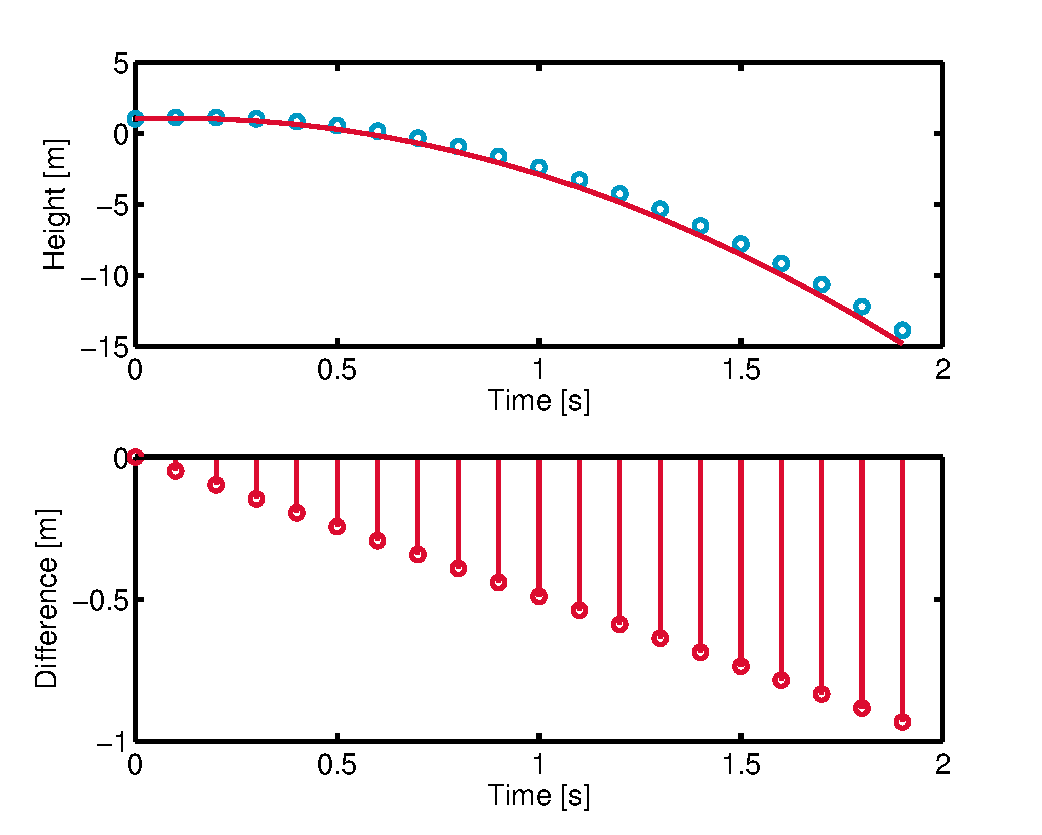
\includegraphics[width=0.8\textwidth]{projectile-utc}
%  \end{center}
%\end{frame}

\section{Conclusions}
\subsection*{Conclusions}
\begin{frame}[fragile]
  \frametitle{In conclusion...}
  \begin{itemize}
    \colorize<1-> \item Algorithm design: define your problem, think ahead, make a scheme, sketch the interplay between variables and functions, then start programming
    \colorize<2-> \item Programming basics: variables, operators and functions, locality of variables, recursive operations
    \colorize<3-> \item Dealing with complex programs, verification of your algorithms, use of the debugger
    \colorize<4-> \item Visualisation: how to make 1D and 2D/3D plots, create a sensible and intuitive presentation of your data.
    \colorize<5-> \item Examples: a few practice cases
  \end{itemize}
\end{frame}

\end{document}


% References
% http://ocw.mit.edu/courses/electrical-engineering-and-computer-science/6-00sc-introduction-to-computer-science-and-programming-spring-2011/unit-1/lecture-1-introduction-to-6.00/
% http://www.greenteapress.com/thinkpython/html/thinkpython002.html
% https://www.youtube.com/channel/UCLMQ21H2ad95faYG3yGCwYA
%http://stackoverflow.com/questions/4227145/in-matlab-are-variables-really-double-precision-by-default
%http://www.exploringbinary.com/why-0-point-1-does-not-exist-in-floating-point/

